\documentclass[11pt,a4paper]{article}

\usepackage[a4paper,margin=2.5cm,top=2.3cm,bottom=2.5cm]{geometry}
\usepackage{amsmath,amsthm,mathtools}
\usepackage{fontspec}
\usepackage{unicode-math}
\setmainfont{texgyrepagella}[Extension=.otf,UprightFont=*-regular,BoldFont=*-bold,ItalicFont=*-italic,BoldItalicFont=*-bolditalic]
\setsansfont{texgyreheros}[Extension=.otf,UprightFont=*-regular,BoldFont=*-bold,ItalicFont=*-italic,BoldItalicFont=*-bolditalic,Scale=0.92]
\setmathfont{texgyrepagella-math.otf}
\usepackage[croatian]{babel}
\usepackage{microtype}
\usepackage{xcolor}
\usepackage{booktabs,tabularx,array}
\usepackage{enumitem}
\usepackage{titlesec}
\usepackage{caption}
\usepackage{tikz}
\usetikzlibrary{arrows.meta,calc}
\usepackage{pgfplots}
\pgfplotsset{compat=1.16}
\usepackage{tcolorbox}
\tcbuselibrary{skins,breakable}
\usepackage[hidelinks]{hyperref}

\definecolor{accent}{HTML}{0F5E63}
\definecolor{muted}{HTML}{55606A}
\definecolor{warn}{HTML}{9A4A12}
\definecolor{c1}{HTML}{0F5E63}
\definecolor{c2}{HTML}{B5651D}
\definecolor{c3}{HTML}{6A4C93}

\titleformat{\part}[display]{\centering\sffamily\Large\bfseries\color{accent}}{\partname~\thepart}{0.4em}{\LARGE}
\titleformat{\section}{\sffamily\large\bfseries\color{accent}}{\thesection.}{0.5em}{}
\titleformat{\subsection}{\sffamily\normalsize\bfseries}{\thesubsection}{0.5em}{}
\titlespacing*{\section}{0pt}{1.4em}{0.5em}
\titlespacing*{\subsection}{0pt}{1em}{0.3em}

\setlength{\parindent}{0pt}
\setlength{\parskip}{0.5em}
\setlist{topsep=0.2em,itemsep=0.15em,leftmargin=1.4em}
\newcolumntype{Y}{>{\raggedright\arraybackslash}X}
\renewcommand{\arraystretch}{1.25}
\captionsetup{font=small,labelfont=bf}
\emergencystretch=1.5em
\widowpenalty=10000
\clubpenalty=10000

\theoremstyle{definition}
\newtheorem{definicija}{Definicija}[section]
\theoremstyle{plain}
\newtheorem{teorem}[definicija]{Teorem}
\newtheorem{lema}[definicija]{Lema}
\newtheorem{propozicija}[definicija]{Propozicija}
\newtheorem{korolar}[definicija]{Korolar}
\theoremstyle{remark}
\newtheorem{napomena}[definicija]{Napomena}
\newtheorem{primjer}[definicija]{Primjer}

\newtcolorbox{ukratko}[1][Ukratko]{enhanced,breakable,colback=accent!5,colframe=accent,
  boxrule=0.6pt,arc=2pt,fonttitle=\sffamily\bfseries\small,title=#1,left=6pt,right=6pt}
\newtcolorbox{oprez}[1][Na obrani pazi]{enhanced,breakable,colback=warn!6,colframe=warn,
  boxrule=0.6pt,arc=2pt,fonttitle=\sffamily\bfseries\small,title=#1,left=6pt,right=6pt}

\newcommand{\R}{\mathbb{R}}
\newcommand{\Rp}{\mathbb{R}_{\geq 0}}
\newcommand{\one}{\mathbf{1}}
\newcommand{\iu}{\mathrm{i}}
\newcommand{\Dkl}[2]{D(#1\,\|\,#2)}
\newcommand{\dkl}[2]{d(#1\,\|\,#2)}
\DeclareMathOperator{\diag}{diag}
\DeclareMathOperator{\dom}{dom}
\DeclareMathOperator*{\argmin}{arg\,min}
\newcommand{\izv}[1]{{\small\color{muted}[#1]}}
\newcommand{\formalno}[1]{{\small\color{muted}\sffamily Formalno: odjeljak~\ref{#1}.}\par}
\newcommand{\intuicija}[1]{{\small\color{muted}\sffamily Intuicija: odjeljak~\ref{#1}.}\par}

\hypersetup{pdftitle={NMF i prepisivanje gitare: skripta za obranu},pdfauthor={Lovro}}

\begin{document}

{\sffamily\LARGE\bfseries\color{accent} NMF i prepisivanje gitare: skripta za obranu\par}
\vspace{0.3em}
{\small\color{muted} Matrične i tenzorske metode u analizi podataka \quad·\quad tema~2 iz prijedloga tema
\quad·\quad radni nacrt, 5.~studenoga 2026.\par}
\vspace{0.8em}

\begin{ukratko}[O ovoj skripti]
\begin{itemize}
\item Skripta pokriva matematiku koju trebamo znati ako odaberemo temu~2 iz prijedloga tema:
  automatsko prepisivanje snimke akustične gitare u note pomoću nenegativne matrične
  faktorizacije (NMF). \textbf{Tema još nije odabrana}, pa ni izbori opisani ovdje (veličina
  prozora, način učenja predložaka, prag) nisu odluke tima, nego prijedlozi.
\item Pretpostavlja se samo preddiplomsko predznanje: linearna algebra, analiza funkcija više
  varijabli i osnovna vjerojatnost. Fourierovu transformaciju, konveksnost, Jensenovu nejednakost
  i uvjete optimalnosti uvodimo u tekstu.
\item \textbf{Dio~I} gradi intuiciju redoslijedom kojim teče projekt: od zvuka do matrice, od
  matrice do faktorizacije, od faktorizacije do nota. \textbf{Dio~II} istim redoslijedom daje
  definicije, tvrdnje i dokaze. Na početku svakog odjeljka stoji poveznica na pripadni odjeljak
  drugog dijela.
\item Oznake L1--L4 odnose se na priložene radove iz vodiča kroz literaturu
  (\nolinkurl{docs/research/LITERATURE.md}). Uz svaku tvrdnju piše odakle je; \emph{vlastiti izvod}
  znači da tvrdnje u tom obliku nema u priloženim radovima. Izvore izvan priloženih radova treba
  pročitati i provjeriti prije citiranja u seminaru.
\item Nijedan eksperiment još nije pokrenut, pa skripta ne sadrži rezultate. Nitko iz tima je još
  nije pregledao.
\end{itemize}
\end{ukratko}

\tableofcontents

% =====================================================================
\part{Intuitivni pregled}
% =====================================================================

\section{Problem: od zvuka do nota}\label{sec:i-problem}
\formalno{sec:f-signal}

Glazbenik svira akustičnu gitaru, a mi imamo samo snimku zvuka. Želimo automatski dobiti popis
odsviranih nota: za svaku notu njezinu \emph{visinu}, \emph{trenutak početka} i \emph{trenutak
kraja}. Takav se popis često crta kao \emph{klavirska rola}: vodoravna os je vrijeme, okomita os
visina tona, a svaka nota je vodoravna crta. Zadatak se zove automatska transkripcija glazbe.

Pitanje teme~2 glasi: \textbf{može li NMF iz snimke prepoznati koje tonove glazbenik svira i kada,
i koliko to dobro radi na gitaristu kojeg model nije vidio tijekom učenja?}

\subsection{Ton, frekvencija i harmonici}

Zvuk je titranje tlaka zraka; mikrofon ga bilježi kao funkciju vremena $x(t)$. Žica koja titra
osnovnom frekvencijom $f_0$ ne proizvodi samo sinusoidu frekvencije $f_0$, nego i njezine
\emph{harmonike}: sinusoide frekvencija $2f_0, 3f_0, 4f_0,\dots$, obično sve slabije. Ton zato u
frekvencijskom prikazu izgleda kao \emph{češalj} (slika~\ref{fig:cesalj}). Položaj zubaca određuje
visinu tona, a njihove relativne visine boju zvuka: ista nota na gitari i klaviru ima zupce na
istim mjestima, ali različitih visina.

Visinu tona zapisujemo cijelim brojem $p$ (MIDI broj). Pripadna osnovna frekvencija je
\[
  f(p) = 440 \cdot 2^{(p-69)/12}\ \text{Hz}.
\]
Susjedne note (razmak od jednog polustepena) razlikuju se faktorom $2^{1/12}\approx 1{,}059$, a
oktava je udvostručenje frekvencije. Gitara u standardnom ugađanju ima prazne žice E2, A2, D3, G3,
B3 i E4 (MIDI 40, 45, 50, 55, 59, 64). Najniži ton E2 ima oko $82{,}4$~Hz. Uz dvadesetak pragova
najviši su tonovi oko MIDI~84 (oko 1047~Hz), pa na gitari postoji nekoliko desetaka mogućih
visina. Točan raspon odredit ćemo iz podataka.

\begin{figure}[ht]
\centering
\begin{tikzpicture}[x=0.012cm,y=1cm]
  \foreach \row/\yy in {0/3.4,1/1.7,2/0} {
    \draw[->,muted] (0,\yy) -- (1050,\yy);
  }
  \node[anchor=east,font=\small] at (-10,3.8) {A2};
  \node[anchor=east,font=\small] at (-10,2.1) {A3};
  \node[anchor=east,font=\small] at (-10,0.4) {A2 + A3};
  \foreach \h in {1,...,9} {
    \pgfmathsetmacro{\hh}{1.2/\h}
    \draw[c1,line width=1.6pt] (110*\h,3.4) -- ++(0,\hh);
    \draw[c1,line width=1.6pt] (110*\h,0) -- ++(0,\hh);
  }
  \foreach \h in {1,...,4} {
    \pgfmathsetmacro{\hh}{0.9/\h}
    \pgfmathsetmacro{\base}{1.2/(2*\h)}
    \draw[c2,line width=1.6pt] (220*\h,1.7) -- ++(0,\hh);
    \draw[c2,line width=1.6pt] (220*\h,\base) -- ++(0,\hh);
  }
  \foreach \f in {0,200,400,600,800,1000} {
    \draw[muted] (\f,0) -- (\f,-0.08) node[below,font=\scriptsize] {\f};
  }
  \node[font=\small,muted] at (525,-0.9) {frekvencija (Hz)};
\end{tikzpicture}
\caption{Idealizirani spektri tona A2 ($f_0=110$~Hz), tona A3 oktavu više ($f_0=220$~Hz) i njihova
zbroja. Svaki harmonik tona A3 pada na parni harmonik tona A2, pa se u zbroju samo neki zupci
povise. Zato je teško razlikovati ,,A2`` od ,,A2 + A3``. Visine zubaca su izmišljene.}
\label{fig:cesalj}
\end{figure}

\subsection{Zašto je to teško}

\begin{itemize}
\item \textbf{Polifonija.} Na gitari često zvuči više nota istodobno (akordi), pa se njihovi
  spektri zbrajaju.
\item \textbf{Preklapanje harmonika.} Nota oktavu iznad dijeli sve svoje harmonike s parnim
  harmonicima niže note (slika~\ref{fig:cesalj}). Kod kvinte treći harmonik niže note gotovo se
  poklapa s drugim harmonikom više; u temperiranom ugađanju razlika je oko 2 centa (cent je
  stoti dio polustepena). Otuda tipične oktavne pogreške.
\item \textbf{Ista visina na različitim žicama.} Primjerice, E4 se može odsvirati na praznoj prvoj
  žici ili na petom pragu druge žice. Zvuk je sličan, ali ne i jednak.
\item \textbf{Promjena kroz vrijeme.} Nakon trzaja ton naglo jača i zatim zamire, a viši harmonici
  zamiru brže od nižih. Spektar jedne note nije stalan.
\end{itemize}

\section{Od zvuka do nenegativne matrice}\label{sec:i-spektrogram}
\formalno{sec:f-signal}

\subsection{Uzorkovanje i Fourierova ideja}

Računalo pohranjuje zvuk kao niz uzoraka $x[\tau]=x(\tau/f_s)$, gdje je $f_s$ frekvencija
uzorkovanja, primjerice $44\,100$ uzoraka u sekundi. Osnovna ideja Fourierove analize jest da se
svaki konačan niz od $N$ uzoraka može zapisati kao zbroj $N$ titraja frekvencija $q f_s/N$,
$q=0,\dots,N-1$. Diskretna Fourierova transformacija (DFT) za svaku od tih frekvencija daje jedan
kompleksan broj. Njegov modul kaže \emph{koliko} te frekvencije ima u isječku, a argument
\emph{u kojoj je fazi}, odnosno koliko je titraj pomaknut u vremenu. Čista sinusoida frekvencije
$f_0$ daje vrh oko indeksa $q\approx f_0 N/f_s$.

\subsection{Prozori i spektrogram}

Glazba se mijenja u vremenu, pa DFT ne računamo na cijeloj snimci, nego na kratkim isječcima.
Uzmemo $N$ uzoraka, pomnožimo ih \emph{prozorom} koji glatko spušta rubove isječka na nulu
(time smanjujemo razlijevanje vrha na susjedne frekvencije), izračunamo DFT, pomaknemo se za $L$
uzoraka i ponovimo. To je \emph{kratkotrajna Fourierova transformacija} (STFT). Module posložimo u
matricu: redak~$i$ odgovara frekvencijskom binu, stupac~$j$ vremenskom okviru. Dobivena matrica
$A$ je \emph{amplitudni spektrogram}. Njezini elementi su moduli, pa su \textbf{nenegativni}.

Duljina prozora nameće kompromis. Razmak susjednih binova je $f_s/N$, a vrh jedne sinusoide kroz
Hannov prozor širok je oko četiri bina. Dvije bliske sinusoide jasno se razdvajaju tek kad im se
frekvencije razlikuju za otprilike dva bina. Dulji prozor znači finije frekvencije, ali grublje
vrijeme:

\begin{center}
\small
\begin{tabular}{@{}rrrr@{}}
\toprule
$N$ (uz $f_s=44\,100$) & razmak binova $f_s/N$ & trajanje prozora & dva bina\\
\midrule
2048 & 21,5 Hz & 46 ms & 43 Hz\\
4096 & 10,8 Hz & 93 ms & 22 Hz\\
8192 & 5,4 Hz & 186 ms & 11 Hz\\
\bottomrule
\end{tabular}
\end{center}

Tonovi E2 i F2 razlikuju se za samo $4{,}9$~Hz. Njihove osnovne frekvencije razdvojio bi tek prozor
od preko trećine sekunde, a brze note traju kraće. Pomažu viši harmonici: $h$-ti harmonici dviju
susjednih nota razlikuju se za $h$ puta više herca. Izbor $N$ i $L$ zato je stvar mjerenja na
podacima za učenje, a ne teorije.

\subsection{Zašto modul i zašto ,,približno zbroj``}

STFT je linearna: transformacija zbroja dvaju signala jednaka je zbroju transformacija. To vrijedi
za kompleksne vrijednosti, a mi koristimo module. Modul zbroja općenito nije zbroj modula
($|z_1+z_2|\leq|z_1|+|z_2|$), osim kad su faze jednake ili kad je jedan od brojeva nula. Dvije
različite note uglavnom imaju energiju u \emph{različitim} binovima, pa je u svakom binu jedan
od dvaju doprinosa gotovo nula i moduli se približno zbrajaju. U binovima u kojima se harmonici
preklapaju to ne vrijedi i model griješi.

Fazu odbacujemo jer se pri pomaku signala u vremenu mijenja, dok modul ostaje gotovo isti. Modul je
stabilan opis toga \emph{koliko čega ima}.

\begin{ukratko}
Snimka postaje matrica $A\in\Rp^{m\times n}$: $m$ frekvencijskih binova, $n$ vremenskih okvira.
Element $a_{ij}$ govori koliko frekvencije $f_i$ ima u okviru~$j$. Spektar zbroja nota približno
je zbroj spektara nota.
\end{ukratko}

\section{Model \texorpdfstring{$A\approx WH$}{A ≈ WH}}\label{sec:i-model}
\formalno{sec:f-nmf}

\subsection{Predlošci i aktivacije}

Pretpostavimo da svaka od $r$ mogućih nota ima stalan spektralni \emph{predložak}
$w_k\in\Rp^m$ (njezin češalj) i da u okviru $j$ zvuči jačinom $h_{kj}\geq0$. Tada je spektar okvira
\[
  a_j \approx \sum_{k=1}^r h_{kj}\, w_k = W h_j,
\]
a za sve okvire odjednom $A\approx WH$. Stupci matrice $W\in\Rp^{m\times r}$ su predlošci, a retci
matrice $H\in\Rp^{r\times n}$ aktivacije nota kroz vrijeme. Matrica $H$ je, dakle, klavirska rola s
jačinama (slika~\ref{fig:model}).

\begin{figure}[ht]
\centering
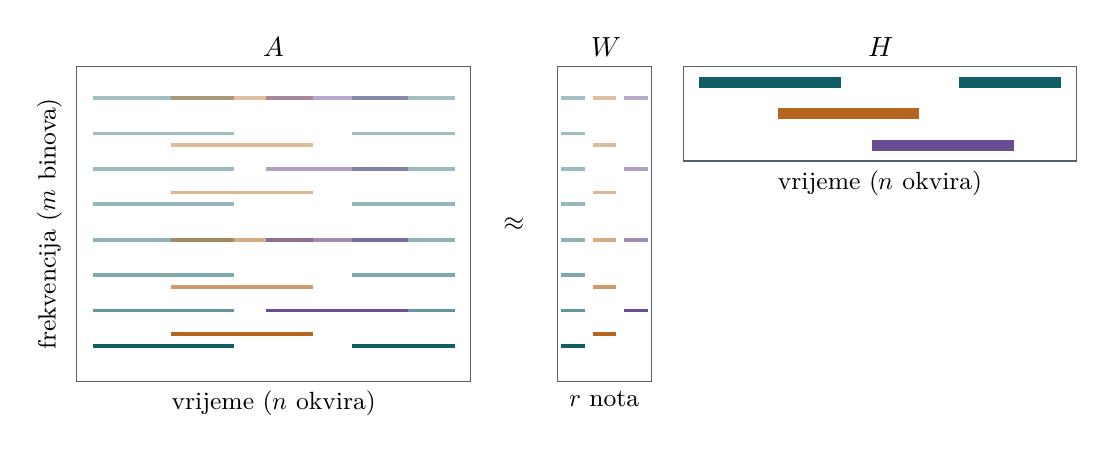
\begin{tikzpicture}[x=1cm,y=1cm]
  \def\fA{0.45}\def\fB{0.6}\def\fC{0.9}
  % A
  \draw[muted] (0,0) rectangle (5,4);
  \foreach \f/\col/\ints in {\fA/c1/{0.2/2.0,3.5/4.8},\fB/c2/{1.2/3.0},\fC/c3/{2.4/4.2}} {
    \foreach \s/\e in \ints {
      \foreach \h in {1,...,8} {
        \pgfmathsetmacro{\yy}{\h*\f}
        \pgfmathsetmacro{\op}{0.3+0.7/\h}
        \ifdim \yy pt<3.95pt
          \draw[\col,line width=1.3pt,opacity=\op] (\s,\yy) -- (\e,\yy);
        \fi
      }
    }
  }
  \node[above] at (2.5,4) {$A$};
  \node[below,font=\small] at (2.5,0) {vrijeme ($n$ okvira)};
  \node[rotate=90,font=\small] at (-0.35,2) {frekvencija ($m$ binova)};
  \node at (5.55,2) {$\approx$};
  % W
  \draw[muted] (6.1,0) rectangle (7.3,4);
  \foreach \f/\col/\k in {\fA/c1/0,\fB/c2/1,\fC/c3/2} {
    \foreach \h in {1,...,8} {
      \pgfmathsetmacro{\yy}{\h*\f}
      \pgfmathsetmacro{\op}{0.3+0.7/\h}
      \ifdim \yy pt<3.95pt
        \draw[\col,line width=1.3pt,opacity=\op] (6.15+0.4*\k,\yy) -- (6.45+0.4*\k,\yy);
      \fi
    }
  }
  \node[above] at (6.7,4) {$W$};
  \node[below,font=\small] at (6.7,0) {$r$ nota};
  % H
  \draw[muted] (7.7,2.8) rectangle (12.7,4);
  \foreach \col/\k/\ints in {c1/0/{0.2/2.0,3.5/4.8},c2/1/{1.2/3.0},c3/2/{2.4/4.2}} {
    \foreach \s/\e in \ints {
      \draw[\col,line width=4pt] (7.7+\s,3.8-0.4*\k) -- (7.7+\e,3.8-0.4*\k);
    }
  }
  \node[above] at (10.2,4) {$H$};
  \node[below,font=\small] at (10.2,2.8) {vrijeme ($n$ okvira)};
\end{tikzpicture}
\caption{Shema modela. Svaka od triju nota ima češalj (stupac od $W$) i razdoblja u kojima zvuči
(redak od $H$). Spektrogram $A$ je zbroj umnožaka. Treća nota (ljubičasta) oktavu je iznad prve
(plave), pa joj svi zupci padaju na zupce prve note. Shema je izmišljena, nisu to stvarni podaci.}
\label{fig:model}
\end{figure}

Red veličine: uz $N=4096$ je $m=2049$, minuta zvuka uz pomak $L=512$ daje nekoliko tisuća okvira,
a $r$ je nekoliko desetaka. Model opisuje $mn$ brojeva s $r(m+n)$ brojeva, dakle sažeto.

\subsection{Zašto nenegativnost}

Zvukovi se u modulu zbrajaju, a ne oduzimaju; aktivacija ,,minus jedan A2`` nema fizikalni smisao.
Lee i Seung (L2) na primjerima pokazuju da nenegativnost vodi na prikaz \emph{po dijelovima}:
lica se rastavljaju na nos, oči i usta, a tekstovi na teme. Kod nas su dijelovi note.

Usporedba sa SVD-om je poučna. Skraćeni SVD daje najbolju aproksimaciju ranga $r$ u Frobeniusovoj
normi i računa se učinkovito (L1, odj.~3). Njegovi vektori, međutim, imaju i negativne elemente:
opisuju cjeline koje se međusobno poništavaju i ne mogu se čitati kao note. NMF zbog dodatnih
ograničenja daje lošiju aproksimaciju u toj normi, ali faktori mogu imati fizikalno značenje, i to
\emph{ako model vrijedi}. Nenegativnost sama po sebi ne jamči smislene komponente.

\subsection{Što je \texorpdfstring{$r$}{r}}

Kod nenadziranog NMF-a rang $r$ treba odabrati, što nije lako (L1, odj.~3). Kod nas $r$ određuje
raspon gitare: jedan predložak po visini tona, ili nekoliko po visini ako želimo razlikovati žice.
To je jedan od razloga za \emph{nadzirano} učenje predložaka (odjeljak~\ref{sec:i-primjena}).

\section{Kako mjeriti koliko je \texorpdfstring{$WH$}{WH} blizu \texorpdfstring{$A$}{A}}\label{sec:i-cilj}
\formalno{sec:f-nmf}

Trebamo mjeru odstupanja koja se zbraja po elementima: $\sum_{i,j} d(a_{ij}\,\|\,b_{ij})$, uz
$B=WH$.

\textbf{Frobeniusova norma}, $d(a\|b)=\frac12(a-b)^2$, poznata je metoda najmanjih kvadrata.
Statistički odgovara pretpostavci da je šum Gaussov i jednako jak u svakom elementu.

\textbf{Generalizirana Kullback–Leiblerova (KL) divergencija} (L3, odj.~3) jest
\[
  d(a\,\|\,b) = a\log\frac{a}{b} - a + b .
\]
Ona je nenegativna i jednaka nuli samo za $a=b$, ali nije simetrična (slika~\ref{fig:kazne}).
Ako model u binu u kojem ima energije ($a>0$) predvidi $b\to0$, kazna raste u beskonačnost: model
ne smije ,,zaboraviti`` energiju. Ako predvidi previše, kazna raste samo linearno.

\begin{figure}[ht]
\centering
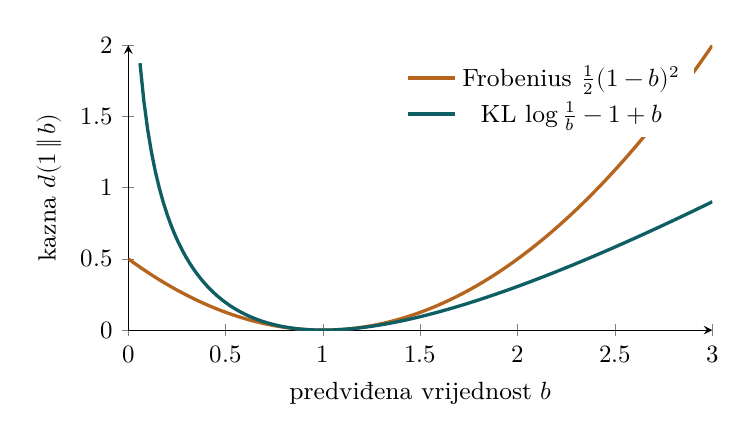
\begin{tikzpicture}
\begin{axis}[width=9cm,height=5.2cm,xmin=0,xmax=3,ymin=0,ymax=2,
  xlabel={predviđena vrijednost $b$},ylabel={kazna $d(1\,\|\,b)$},
  legend style={draw=none,font=\small,at={(0.97,0.97)},anchor=north east},
  tick label style={font=\small},label style={font=\small},axis lines=left]
  \addplot[c2,very thick,domain=0:3,samples=100] {0.5*(1-x)^2};
  \addlegendentry{Frobenius $\tfrac12(1-b)^2$}
  \addplot[c1,very thick,domain=0.06:3,samples=150] {-ln(x)-1+x};
  \addlegendentry{KL $\log\frac1b-1+b$}
\end{axis}
\end{tikzpicture}
\caption{Kazna za jedan element uz izmjereno $a=1$. Oko $b=1$ obje se ponašaju jednako, ali KL
jako kažnjava podcjenjivanje.}
\label{fig:kazne}
\end{figure}

\textbf{Ljestvica.} Najvažnija razlika je u tome kako se kazna mijenja s glasnoćom. Pogledajmo
pogrešku od 10~\% u tihom i u stotinu puta glasnijem binu:

\begin{center}
\small
\begin{tabular}{@{}lrrr@{}}
\toprule
& $a=1$, $b=1{,}1$ & $a=100$, $b=110$ & omjer\\
\midrule
Frobenius $\tfrac12(a-b)^2$ & 0,005 & 50 & $10^4$\\
generalizirana KL & 0,0047 & 0,47 & $10^2$\\
\bottomrule
\end{tabular}
\end{center}

Frobeniusova kazna raste s kvadratom glasnoće, a KL linearno. Glazbeni spektrogram ima velik
dinamički raspon: osnovni ton glasne note može biti stotinama puta jači od visokog harmonika tihe
note. Uz Frobeniusovu normu algoritam se gotovo samo trudi oko najglasnijih binova, a KL ravnomjernije
raspoređuje pažnju. Itakura–Saitova divergencija, koju L1 spominje za analizu glazbe, potpuno je
neovisna o ljestvici. Ne koristimo je, ali je dobra tema za pitanje ,,zašto baš KL``.

\textbf{Statistička interpretacija.} Minimizacija KL divergencije jednaka je traženju najveće
izglednosti uz pretpostavku da je svaki $a_{ij}$ Poissonova slučajna varijabla s očekivanjem
$(WH)_{ij}$ (L2, jedn.~(2)). To je motivacija, a ne dokaz da je KL ,,ispravna`` za naše podatke:
moduli spektrograma nisu cijeli brojevi. Pravi test je kvaliteta transkripcije, pa u planu
eksperimenata postoji usporedba s Frobeniusovom normom.

\section{Kako naći \texorpdfstring{$W$}{W} i \texorpdfstring{$H$}{H}}\label{sec:i-algoritam}
\formalno{sec:f-mu}

\subsection{Težak problem s laganim dijelovima}

Rješavamo
\[
  \min_{W\geq0,\ H\geq0} \Dkl{A}{WH}.
\]
Taj problem je \emph{nekonveksan}: ima mnogo minimuma (već zbog skaliranja, odjeljak~\ref{sec:i-jamstva})
i može imati lokalne minimume i sedla. U općem slučaju NMF je NP-težak (L1, odj.~3), pa ne
očekujemo algoritam koji uvijek nalazi globalni minimum. Međutim, \textbf{kad je $W$ fiksiran,
problem po $H$ je konveksan} (L3, odj.~3), a u konveksnom problemu svaki je lokalni minimum
globalni. Isto vrijedi za $W$ uz fiksiran $H$. Zato algoritam \emph{alternira}: malo popravi $H$,
pa malo popravi $W$, i tako redom.

\subsection{Multiplikativno pravilo i kako ga čitati}

Pravilo za $H$ (L3, teorem~2) glasi
\[
  h_{kj} \leftarrow h_{kj}\cdot
  \frac{\sum_i w_{ik}\,\dfrac{a_{ij}}{(WH)_{ij}}}{\sum_i w_{ik}} .
\]
Omjer $a_{ij}/(WH)_{ij}$ veći je od $1$ kad model u binu $i$ okvira $j$ objašnjava premalo
energije, a manji od $1$ kad objašnjava previše. Faktor kojim množimo $h_{kj}$ ponderirani je
prosjek tih omjera, a težine su predložak $w_k$: gledaju se samo binovi u kojima nota $k$ ima
harmonike. Ako je u tim binovima energija u prosjeku premalo objašnjena, aktivacija note raste, a
ako je previše objašnjena, pada. Kad model savršeno objašnjava podatke, svi su omjeri $1$ i ništa
se ne mijenja. Pravilo za $W$ je analogno.

Pravilo je zapravo korak gradijentnog spusta u kojem svaki element ima svoju duljinu koraka,
odabranu tako da se oduzimanje pokrati i ostane samo množenje. Zato nenegativnost ostaje sama od
sebe, bez projekcija, i ne treba ručno birati duljinu koraka.

\subsection{Zašto se funkcija cilja ne povećava}

Ključna ideja zove se \emph{majorizacija–minimizacija} (slika~\ref{fig:mm}). U trenutnoj točki
$h^t$ konstruiramo jednostavnu funkciju $G(\cdot,h^t)$ koja leži iznad funkcije cilja $F$ i dodiruje
je u $h^t$. Zatim minimiziramo $G$ umjesto $F$. Tada
\[
  F(h^{t+1}) \leq G(h^{t+1},h^t) \leq G(h^t,h^t) = F(h^t).
\]
Za KL divergenciju takva se $G$ dobije iz Jensenove nejednakosti za logaritam, a njezin minimum je
upravo multiplikativno pravilo (L3, odj.~6). Cijeli dokaz je u odjeljku~\ref{sec:f-monotonost}.

\begin{figure}[ht]
\centering
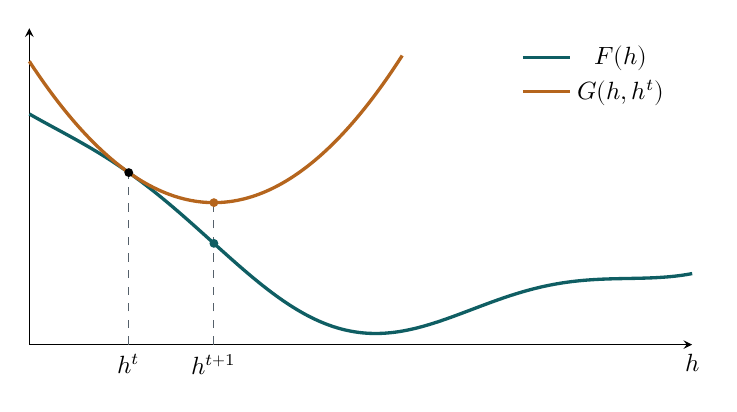
\begin{tikzpicture}
\begin{axis}[width=10cm,height=5.6cm,xmin=0,xmax=4,ymin=0.4,ymax=1.65,
  axis lines=left,xtick=\empty,ytick=\empty,xlabel={$h$},clip=false,x label style={at={(axis description cs:1,0)},anchor=north},
  label style={font=\small},legend style={draw=none,font=\small,at={(0.98,0.98)},anchor=north east}]
  \addplot[c1,very thick,domain=0:4,samples=200] {0.5+0.12*(x-2.6)^2+0.1*sin(deg(2.5*x))};
  \addlegendentry{$F(h)$}
  \addplot[c2,very thick,domain=0:2.25,samples=100] {1.07975-0.46232*(x-0.6)+0.45*(x-0.6)^2};
  \addlegendentry{$G(h,h^t)$}
  \draw[dashed,muted] (axis cs:0.6,0.4) -- (axis cs:0.6,1.07975);
  \draw[dashed,muted] (axis cs:1.1137,0.4) -- (axis cs:1.1137,0.96101);
  \fill[black] (axis cs:0.6,1.07975) circle (1.6pt);
  \fill[c2] (axis cs:1.1137,0.96101) circle (1.6pt);
  \fill[c1] (axis cs:1.1137,0.80008) circle (1.6pt);
  \node[below,font=\small] at (axis cs:0.6,0.4) {$h^t$};
  \node[below,font=\small] at (axis cs:1.1137,0.4) {$h^{t+1}$};
\end{axis}
\end{tikzpicture}
\caption{Majorizacija–minimizacija. Pomoćna funkcija $G$ dodiruje $F$ u $h^t$ i nigdje nije ispod
nje. Njezin minimum $h^{t+1}$ zato ne može povećati $F$. Funkcije su ilustrativne.}
\label{fig:mm}
\end{figure}

\subsection{Mali primjer}

Neka postoje dva bina i dva predloška: $w_1=(1,1)$ je nota s energijom u oba bina, a $w_2=(1,0)$
nota samo u prvom. Izmjereno je $a=(2,1)=w_1+w_2$, pa je točno rješenje $h=(1,1)$ uz $D=0$.
Krenemo li od $h^0=(1,\ 1/5)$, multiplikativno pravilo daje
$D=0{,}2217 \to 0{,}0770 \to 0{,}0627 \to 0{,}0491 \to \cdots \to 0$
(primjer~\ref{pr:iteracije}). Vrijednost pada u svakom koraku, ali sve sporije. Multiplikativna
pravila su poznata po sporosti (L1, odj.~3.1.2; L4, odj.~3.1).

\section{Što je zajamčeno, a što nije}\label{sec:i-jamstva}
\formalno{sec:f-konvergencija}

Ovo je najvažniji odjeljak za obranu. Lako je reći više nego što je dokazano.

\begin{center}
\small
\begin{tabularx}{\linewidth}{@{}Y>{\raggedright\arraybackslash}p{3.4cm}>{\raggedright\arraybackslash}p{3.2cm}@{}}
\toprule
\textbf{Tvrdnja} & \textbf{Vrijedi?} & \textbf{Izvor}\\
\midrule
Funkcija cilja se ni u jednom koraku ne povećava & Da, uz blage pretpostavke & L3, teorem 2\\
Niz vrijednosti funkcije cilja konvergira & Da (monoton, omeđen nulom) & elementarno\\
Iterati $(W^t,H^t)$ konvergiraju & Nije dokazano & L4, odj.~3.1\\
Granična točka je stacionarna & Dokazano samo za točke s pozitivnim elementima & L4, odj.~3.1; ovdje prop.~\ref{prop:pozitivna-granica}\\
Dobivamo lokalni minimum & Nije dokazano (L3 to tvrdi, L4 ispravlja) & L3, odj.~6; L4, odj.~3.1\\
Dobivamo globalni minimum & Općenito ne & L1, odj.~3\\
Faktori su jedinstveni & Ne & L1, odj.~3\\
Uz fiksiran $W$ problem po $H$ je konveksan & Da & L3, odj.~3\\
\bottomrule
\end{tabularx}
\end{center}

\textbf{Zamka s nulama.} Ako $h_{kj}$ u nekom koraku postane $0$, multiplikativno pravilo ga više
nikad ne pomiče. Algoritam tako može zapeti u točki koja nije ni stacionarna. U malom primjeru,
krenemo li od $h^0=(1,0)$, već u prvom koraku stižemo u $(3/2,0)$ i tamo ostajemo zauvijek, uz
$D\approx0{,}17$, iako je minimum $0$ (primjer~\ref{pr:zapinjanje}). Pouka: inicijaliziramo
pozitivnim brojevima. Nule koje stavljamo namjerno, kao u odjeljku~\ref{sec:i-primjena}, koriste baš
to svojstvo.

\textbf{Nejedinstvenost.} Za svaku pozitivnu dijagonalnu matricu $\Lambda$ vrijedi
$WH=(W\Lambda)(\Lambda^{-1}H)$, a i stupci od $W$ mogu se permutirati zajedno s retcima od $H$.
Skaliranje uklanjamo normalizacijom: zbroj svakog stupca od $W$ postavimo na $1$, a $H$
odgovarajuće prilagodimo. Tada je $h_{kj}$ ukupna ,,masa`` note $k$ u okviru $j$. Permutacija kod
nas ne smeta jer predloške učimo iz oznaka, pa je stupac $k$ po konstrukciji nota $k$.

\begin{oprez}
\begin{itemize}
\item Ne govori ,,algoritam konvergira lokalnom minimumu``. Reci: ,,funkcija cilja ne raste; ako
  iterati konvergiraju prema točki s pozitivnim elementima, ta je točka stacionarna``.
\item Stacionarna točka nije nužno lokalni minimum. Primjerice, $(W,H)=(0,0)$ je stacionarna točka
  Frobeniusove funkcije cilja (primjer~\ref{pr:nula-stacionarna}).
\item Nenegativnost ne jamči da su predlošci ,,prave note``; to provjeravamo na podacima.
\item Težine $h_{kj}$ nisu vjerojatnosti.
\end{itemize}
\end{oprez}

\section{Od teorije do transkripcije}\label{sec:i-primjena}
\formalno{sec:f-primjena}

\subsection{Podaci i podjela}

Skup GuitarSet (CC BY 4.0) ima 360 snimaka šest gitarista s označenim notama. Predloške učimo na
pet gitarista, a transkripciju provjeravamo na šestom, i to ponavljamo za svakog gitarista (šest
podjela). Tako mjerimo radi li metoda na sviraču kojeg nije vidjela.

\subsection{Učenje predložaka (prijedlog, nije odluka)}

\textbf{Maskirani NMF.} Za snimke za učenje iz oznaka znamo koja nota zvuči u kojem okviru. Tu
informaciju zapišemo kao matricu $M\in\{0,1\}^{r\times n}$. Matricu $H$ inicijaliziramo pozitivnim
brojevima samo tamo gdje je $M_{kj}=1$, a nulama drugdje. Budući da multiplikativno pravilo čuva
nule, aktivacija note koja ne svira ostaje $0$. Algoritam mora objasniti spektar samo notama koje
stvarno zvuče, i tako uči njihove predloške. Teorem o nerastu i dalje vrijedi
(propozicija~\ref{prop:maska}). Dvije praktične zamke:
\begin{itemize}
\item Okvir u kojem ne svira nijedna nota, a ima malo šuma, daje beskonačnu divergenciju. Treba
  dodati jednu komponentu za pozadinski šum koja je uvijek aktivna ili takve okvire izbaciti.
\item Notu koja se u skupu za učenje ne pojavljuje nije moguće naučiti.
\end{itemize}
\textbf{Jednostavnija mogućnost:} predložak note je prosjek normaliziranih spektara okvira u kojima
svira samo ta nota. Oba načina mogu se proširiti na više predložaka po visini, primjerice po žici.

\subsection{Transkripcija nove snimke}

Za snimku novog gitarista izračunamo spektrogram $A'$, \textbf{fiksiramo naučeni $W$} i rješavamo
samo $\min_{H\geq0}\Dkl{A'}{WH}$. Taj je problem konveksan: svaki lokalni minimum je globalni, pa
za razliku od punog problema nema lošijih lokalnih minimuma u kojima bismo mogli zapeti. Zatim:
\begin{enumerate}
\item notu $k$ proglasimo aktivnom u okviru $j$ ako je $h_{kj}$ iznad praga $\theta$;
\item uzastopne aktivne okvire spojimo u jednu notu s početkom i krajem;
\item odbacimo prekratke note.
\end{enumerate}
Prag $\theta$ i najmanju duljinu note biramo na gitaristima za učenje, \textbf{nikad na testnom}.

\subsection{Vrednovanje}

Procijenjena nota je \emph{pogodak} ako ima istu visinu kao neka stvarna nota i počinje dovoljno blizu
njezinu početku; uobičajena tolerancija je 50~ms. Svaka stvarna nota smije se upariti s najviše
jednom procijenjenom. Tada je
\[
  P=\frac{\text{pogoci}}{\text{sve procijenjene note}},\qquad
  R=\frac{\text{pogoci}}{\text{sve stvarne note}},\qquad
  F_1=\frac{2PR}{P+R}.
\]
Preciznost $P$ kažnjava izmišljene note, a odziv $R$ propuštene. Prijavljujemo $F_1$ za svakog od
šest gitarista i prosjek, a ne samo najbolji slučaj. Uspoređujemo se s istim postupkom uz
Frobeniusovu normu i s jednostavnim odabirom spektralnih vrhova.

\subsection{Što očekivati}

Očekujemo oktavne pogreške, probleme s akordima, s istom notom na različitim žicama i sa zamiranjem
tona. Skroman $F_1$ legitiman je rezultat ako je pošteno izmjeren i analiziran.

\section{Sažetak u deset rečenica}\label{sec:i-sazetak}

\begin{ukratko}[Za ponavljanje prije obrane]
\begin{enumerate}
\item Snimku pretvaramo u amplitudni spektrogram $A\geq0$; retci su frekvencije, stupci vrijeme.
\item Spektar više nota približno je zbroj spektara nota jer se njihova energija uglavnom nalazi u
  različitim binovima.
\item Model $A\approx WH$: stupci od $W$ su predlošci nota, retci od $H$ njihove aktivacije.
\item Odstupanje mjerimo generaliziranom KL divergencijom koja, za razliku od Frobeniusove norme,
  ne pušta da najglasniji binovi dominiraju.
\item Puni problem je nekonveksan i NP-težak, ali je uz fiksiran $W$ konveksan po $H$.
\item Multiplikativna pravila su skalirani gradijentni koraci koji automatski čuvaju nenegativnost.
\item Funkcija cilja ne raste jer je svaki korak minimum pomoćne funkcije koja leži iznad nje.
\item Nije dokazano da iterati konvergiraju, ni da je granica lokalni minimum; nule ostaju nule.
\item Predloške učimo iz označenih snimaka, a novu snimku obrađujemo rješavanjem konveksnog
  problema po $H$ i pragom.
\item Uspjeh mjerimo s $F_1$ na razini nota, odvojeno za svakog gitarista kojeg model nije vidio.
\end{enumerate}
\end{ukratko}

% =====================================================================
\part{Formalni pregled}
% =====================================================================

\section{Oznake i alati}\label{sec:f-oznake}

\subsection{Matrice}

$\Rp^{m\times n}$ je skup realnih $m\times n$ matrica s nenegativnim elementima; $A\geq0$ i $A>0$
znače da su svi elementi nenegativni, odnosno pozitivni. Stupac $j$ matrice $A$ označavamo s
$a_j$, a redak $k$ matrice $H$ s $H_{k,:}$. Za matrice istih dimenzija
\[
  (X\odot Y)_{ij}=x_{ij}y_{ij},\qquad (X\oslash Y)_{ij}=x_{ij}/y_{ij},
\]
a $\one$ je matrica (ili vektor) jedinica odgovarajućih dimenzija. Skalarni produkt matrica je
$\langle X,Y\rangle=\sum_{ij}x_{ij}y_{ij}=\operatorname{tr}(X^TY)$, a Frobeniusova norma
$\|X\|_F=\langle X,X\rangle^{1/2}$.

Za funkciju $f$ matrične varijable $X$, gradijent $\nabla_X f$ je matrica istih dimenzija kao $X$
s elementima $\partial f/\partial x_{ij}$. Ekvivalentno, $f(X+\varepsilon E)=f(X)+\varepsilon\langle
\nabla_X f, E\rangle+o(\varepsilon)$ za svaku matricu smjera $E$.

\subsection{Konveksnost}

Skup $C$ je konveksan ako sadrži dužinu između bilo kojih dviju svojih točaka. Funkcija
$f\colon C\to\R$ je konveksna ako je $f((1-t)x+ty)\leq(1-t)f(x)+tf(y)$ za sve $x,y\in C$ i
$t\in[0,1]$, a konkavna ako je $-f$ konveksna. Koristimo sljedeće poznate činjenice:
\begin{itemize}
\item dvaput diferencijabilna funkcija na otvorenom konveksnom skupu konveksna je ako i samo ako joj
  je Hesseova matrica pozitivno semidefinitna u svakoj točki;
\item zbroj konveksnih funkcija je konveksan, a $x\mapsto f(Mx+c)$ je konveksna ako je $f$ konveksna;
\item $-\log$ je konveksna na $(0,\infty)$ jer je $(-\log x)''=1/x^2>0$, pa je $\log$ konkavan.
\end{itemize}

\begin{propozicija}\label{prop:lokalni-globalni}
Ako je $f$ konveksna na konveksnom skupu $C$, svaki lokalni minimum od $f$ na $C$ je globalni.
\end{propozicija}
\begin{proof}
Neka je $x$ lokalni minimum i neka postoji $y\in C$ s $f(y)<f(x)$. Za $t\in(0,1]$ je
$f(x+t(y-x))\leq(1-t)f(x)+tf(y)<f(x)$, a točke $x+t(y-x)$ su za mali $t$ po volji blizu $x$.
To je u kontradikciji s lokalnom minimalnošću.
\end{proof}

\begin{propozicija}[Jensenova nejednakost]\label{prop:jensen}
Ako je $\varphi$ konkavna, $z_1,\dots,z_s$ iz njezine domene, a $\lambda_k\geq0$ uz
$\sum_k\lambda_k=1$, tada je $\varphi\bigl(\sum_k\lambda_kz_k\bigr)\geq\sum_k\lambda_k\varphi(z_k)$.
\end{propozicija}
\begin{proof}
Za $s=2$ to je definicija konkavnosti. Korak indukcije: za $\lambda_s<1$ zapišemo
$\sum_k\lambda_kz_k=(1-\lambda_s)\sum_{k<s}\frac{\lambda_k}{1-\lambda_s}z_k+\lambda_sz_s$ i primijenimo
slučaj $s=2$, a zatim pretpostavku indukcije.
\end{proof}

Koristit ćemo i činjenicu da monoton i omeđen niz realnih brojeva konvergira.

\section{Signal, DFT i spektrogram}\label{sec:f-signal}
\intuicija{sec:i-spektrogram}

U ovom odjeljku $\iu$ je imaginarna jedinica, a frekvencijske binove indeksiramo s $q$ jer počinju
od nule.

\begin{definicija}[DFT]
Za $y\in\mathbb{C}^N$ diskretna Fourierova transformacija je
\[
  \hat y[q]=\sum_{\tau=0}^{N-1}y[\tau]\,e^{-2\pi\iu\,q\tau/N},\qquad q=0,\dots,N-1.
\]
\end{definicija}

\begin{propozicija}\label{prop:dft}
\begin{enumerate}[label=(\alph*)]
\item DFT je linearna: $\widehat{\alpha y+\beta z}=\alpha\hat y+\beta\hat z$.
\item Vrijedi formula inverzije $y[\tau]=\frac1N\sum_{q=0}^{N-1}\hat y[q]\,e^{2\pi\iu\,q\tau/N}$. Dakle
  $y$ je kombinacija $N$ kompleksnih titraja; uz frekvenciju uzorkovanja $f_s$ titraj s indeksom
  $q$ ima frekvenciju $qf_s/N$.
\item Ako je $y$ realan, tada je $\hat y[N-q]=\overline{\hat y[q]}$, pa je za paran $N$ dovoljno
  promatrati $q=0,\dots,N/2$.
\end{enumerate}
\end{propozicija}
\begin{proof}
(a) je očito. (b) slijedi iz $\sum_{\tau=0}^{N-1}e^{2\pi\iu(q-q')\tau/N}=N$ za $q=q'$ i $0$ inače
(zbroj geometrijskog niza). (c) $e^{-2\pi\iu(N-q)\tau/N}=e^{2\pi\iu q\tau/N}=\overline{e^{-2\pi\iu
q\tau/N}}$, a $y[\tau]$ su realni.
\end{proof}

\begin{definicija}[STFT i spektrogram]\label{def:spektrogram}
Neka je $x[\tau]$ signal uzorkovan frekvencijom $f_s$, $N$ paran broj, $L$ pomak, a
$g\colon\{0,\dots,N-1\}\to[0,\infty)$ prozor, npr.\ Hannov, $g[\tau]=\sin^2(\pi\tau/N)$. Za okvir $j=0,\dots,n-1$ i
bin $q=0,\dots,N/2$:
\[
  X[q,j]=\sum_{\tau=0}^{N-1}x[jL+\tau]\,g[\tau]\,e^{-2\pi\iu\,q\tau/N},\qquad A_{qj}=|X[q,j]|.
\]
Matrica $A\in\Rp^{m\times n}$, $m=N/2+1$, je amplitudni spektrogram. Bin $q$ odgovara frekvenciji
$qf_s/N$, a okvir $j$ trenutku $(jL+N/2)/f_s$ (sredina prozora).
\end{definicija}

\begin{propozicija}[sinusoida kroz prozor; vlastiti izvod]\label{prop:sinusoida}
Neka je $x[\tau]=c\cos(2\pi f_0\tau/f_s+\phi)$ uz $c>0$, neka je $\kappa_0=f_0N/f_s$ i
$\hat G(\nu)=\sum_{\tau=0}^{N-1}g[\tau]e^{-2\pi\iu\nu\tau/N}$ za realni $\nu$. Tada je
\[
  X[q,j]=\tfrac c2 e^{\iu\phi_j}\,\hat G(q-\kappa_0)+\tfrac c2 e^{-\iu\phi_j}\,\hat G(q+\kappa_0),
  \qquad \phi_j=\phi+2\pi f_0jL/f_s .
\]
Pritom je $|\hat G(\nu)|\leq\hat G(0)=\sum_\tau g[\tau]$.
\end{propozicija}
\begin{proof}
Napišemo $\cos\theta=\frac12(e^{\iu\theta}+e^{-\iu\theta})$ uz
$\theta=\phi_j+2\pi\kappa_0\tau/N$, uvrstimo u definiciju i grupiramo eksponente. Nejednakost je
nejednakost trokuta uz $g\geq0$.
\end{proof}

\begin{napomena}
Za Hannov prozor je $\hat G(0)=N/2$, a $\hat G(\nu)=0$ za cijele $|\nu|\geq2$; glavni vrh zauzima
interval $(\kappa_0-2,\kappa_0+2)$, dakle oko četiri bina. Ako $\kappa_0$ nije blizu $0$ ni $N/2$,
drugi je član zanemariv, pa je $A_{qj}\approx\frac c2|\hat G(q-\kappa_0)|$. To ne ovisi o fazi
$\phi_j$ i zato je modul stabilan kroz okvire. Harmonijski ton
$\sum_h c_h\cos(2\pi hf_0\tau/f_s+\phi_h)$ po linearnosti daje vrhove oko $h\kappa_0$, dakle češalj.
Dvije sinusoide jasno se razlikuju otprilike kad je $|\kappa_1-\kappa_2|\gtrsim2$, tj.\
$|f_1-f_2|\gtrsim2f_s/N$. To je pravilo iskustva, a ne teorem.
\end{napomena}

\begin{propozicija}[zbrajanje modula]\label{prop:zbrajanje}
Za $z_1,z_2\in\mathbb{C}$ je $|z_1+z_2|\leq|z_1|+|z_2|$, s jednakošću ako i samo ako je jedan od njih
$0$ ili imaju isti argument. Nadalje,
$|z_1+z_2|^2=|z_1|^2+|z_2|^2+2|z_1||z_2|\cos\Delta$, gdje je $\Delta$ razlika argumenata. Ako je
$\Delta$ uniformno distribuiran na $[0,2\pi)$, tada je $\mathbb{E}|z_1+z_2|^2=|z_1|^2+|z_2|^2$.
\end{propozicija}
\begin{proof}
Prva tvrdnja je nejednakost trokuta u $\mathbb{C}$. Druga slijedi iz
$|z_1+z_2|^2=(z_1+z_2)\overline{(z_1+z_2)}$. Za treću je $\mathbb{E}\cos\Delta=0$.
\end{proof}

Posljedica: spektrogram zbroja nota je \emph{točno} zbroj spektrograma samo ako note nemaju energiju
u istim binovima ili ako su im faze jednake. Za kvadrate modula zbroj vrijedi u očekivanju uz
nasumične faze. Model $A\approx WH$ je stoga aproksimacija, najlošija u binovima u kojima se
harmonici preklapaju.

\section{NMF i funkcije cilja}\label{sec:f-nmf}
\intuicija{sec:i-model}

Od sada retke od $A$ indeksiramo s $i=1,\dots,m$, stupce s $j=1,\dots,n$, a komponente s
$k=1,\dots,r$.

\begin{definicija}[NMF]
Za $A\in\Rp^{m\times n}$ i $r\in\mathbb{N}$ tražimo $W\in\Rp^{m\times r}$ i $H\in\Rp^{r\times n}$
koji minimiziraju odabranu mjeru odstupanja između $A$ i $WH$. Promatramo
\[
  f_F(W,H)=\tfrac12\|A-WH\|_F^2\qquad\text{i}\qquad f_{KL}(W,H)=\Dkl{A}{WH}.
\]
\end{definicija}

\begin{definicija}[generalizirana KL divergencija; L3, jedn.~(3)]
Za $A,B\geq0$ istih dimenzija je $\Dkl{A}{B}=\sum_{ij}\dkl{a_{ij}}{b_{ij}}$, gdje je
\[
  \dkl{a}{b}=a\log\frac ab-a+b,
\]
uz dogovor $\dkl{0}{b}=b$ i $\dkl{a}{0}=+\infty$ za $a>0$.
\end{definicija}

\begin{propozicija}\label{prop:kl-nenegativna}
$\Dkl{A}{B}\geq0$, s jednakošću ako i samo ako je $A=B$.
\end{propozicija}
\begin{proof}
Dovoljno je promatrati jedan element. Za $a=0$ je $d=b\geq0$, s jednakošću ako i samo ako je
$b=0$. Za $a>0$ i $b=0$ je $d=\infty$. Za $a,b>0$ zapišemo $\dkl ab=b\,\psi(a/b)$ uz
$\psi(x)=x\log x-x+1$. Vrijedi $\psi'(x)=\log x$ i $\psi''(x)=1/x>0$, pa je $\psi$ strogo konveksna s
jedinim minimumom u $x=1$, gdje je $\psi(1)=0$. Dakle $d\geq0$, s jednakošću ako i samo ako je $a=b$.
\end{proof}

\begin{propozicija}[ljestvica; vlastiti izvod]\label{prop:ljestvica}
Za $\lambda>0$ je $\Dkl{\lambda A}{\lambda B}=\lambda\Dkl AB$ i $\|\lambda A-\lambda B\|_F^2=\lambda^2\|A-B\|_F^2$.
\end{propozicija}
\begin{proof}
Izravno iz definicija, jer je $\log\frac{\lambda a}{\lambda b}=\log\frac ab$.
\end{proof}

\begin{napomena}
Itakura–Saitova divergencija $\frac ab-\log\frac ab-1$ ne mijenja se pri skaliranju. L1 (odj.~3) je
navodi za analizu glazbe i upućuje na Févottea i suradnike [FBD]. U ovoj temi je ne koristimo.
\end{napomena}

\begin{propozicija}[Poissonov model; usp.\ L2, jedn.~(2)]\label{prop:poisson}
Neka su $a_{ij}\in\{0,1,2,\dots\}$ nezavisne Poissonove slučajne varijable s parametrima
$b_{ij}=(WH)_{ij}>0$. Tada je
\[
  -\log\mathbb{P}(A\mid W,H)=\Dkl{A}{WH}+c(A),
\]
gdje $c(A)$ ne ovisi o $W$ i $H$. Minimizacija $f_{KL}$ jednaka je maksimizaciji izglednosti.
\end{propozicija}
\begin{proof}
$\mathbb{P}(A\mid W,H)=\prod_{ij}b_{ij}^{a_{ij}}e^{-b_{ij}}/a_{ij}!$, pa je
$-\log\mathbb{P}=\sum_{ij}(b_{ij}-a_{ij}\log b_{ij}+\log a_{ij}!)$. Oduzmemo
$\Dkl AB=\sum_{ij}(a_{ij}\log a_{ij}-a_{ij}\log b_{ij}-a_{ij}+b_{ij})$ i dobijemo
$c(A)=\sum_{ij}(\log a_{ij}!-a_{ij}\log a_{ij}+a_{ij})$.
\end{proof}

\begin{propozicija}[Gaussov model]
Ako je $a_{ij}=(WH)_{ij}+\varepsilon_{ij}$ uz nezavisne $\varepsilon_{ij}\sim\mathcal N(0,\sigma^2)$, tada
je $-\log p(A\mid W,H)=\sigma^{-2}f_F(W,H)+\text{konst}$.
\end{propozicija}
\begin{proof}
Logaritam umnoška gustoća $(2\pi\sigma^2)^{-1/2}\exp(-(a_{ij}-b_{ij})^2/(2\sigma^2))$.
\end{proof}

\begin{napomena}
Moduli spektrograma nisu cijeli brojevi ni Poissonove varijable, pa propozicija~\ref{prop:poisson}
samo motivira izbor KL divergencije. Odluku o funkciji cilja opravdava usporedba na podacima.
\end{napomena}

\section{Struktura problema}\label{sec:f-struktura}
\intuicija{sec:i-algoritam}

\begin{propozicija}[nejedinstvenost; L1, odj.~3]\label{prop:nejedinstvenost}
Ako je $P$ matrica permutacije, a $\Lambda$ dijagonalna matrica s pozitivnom dijagonalom, tada su
$W'=WP\Lambda\geq0$ i $H'=\Lambda^{-1}P^TH\geq0$ te $W'H'=WH$.
\end{propozicija}
\begin{proof}
$P\Lambda\Lambda^{-1}P^T=PP^T=I$; množenje nenegativnih matrica s $P$ i pozitivnom dijagonalom
čuva nenegativnost.
\end{proof}

\begin{napomena}
Mogu postojati i druge invertibilne $Q$ s $WQ\geq0$ i $Q^{-1}H\geq0$; tada su faktorizacije
bitno različite, s različitom interpretacijom (L1, odj.~3, s primjerom $3\times4$). Kod nas
nadzirano učenje određuje poredak stupaca, a normalizacija skaliranje.
\end{napomena}

\begin{propozicija}[normalizacija]\label{prop:normalizacija}
Neka $W$ nema nul-stupac, $s_k=\sum_iw_{ik}$ i $S=\diag(s)$. Za $W'=WS^{-1}$ i $H'=SH$ vrijedi
$W'H'=WH$, zbroj svakog stupca od $W'$ je $1$ i $h'_{kj}=\sum_i w_{ik}h_{kj}$. Vrijednosti funkcija
cilja se ne mijenjaju.
\end{propozicija}
\begin{proof}
Poseban slučaj propozicije~\ref{prop:nejedinstvenost} uz $P=I$, $\Lambda=S^{-1}$.
\end{proof}

\begin{primjer}[nekonveksnost; vlastiti izvod]\label{pr:nekonveksnost}
Neka je $m=n=r=1$ i $a=1$. Tada je na $(0,\infty)^2$
\[
  f(w,h)=\dkl{1}{wh}=-\log w-\log h-1+wh,\qquad
  \nabla^2 f=\begin{pmatrix}1/w^2&1\\1&1/h^2\end{pmatrix}.
\]
Determinanta $1/(w^2h^2)-1$ negativna je za $wh>1$, pa Hesseova matrica tamo ima negativnu
svojstvenu vrijednost i $f$ nije konveksna. Skup minimuma $\{wh=1\}$ je hiperbola: beskonačno mnogo
minimuma, što je upravo nejedinstvenost skaliranja. Za Frobeniusovu normu, $f=\frac12(1-wh)^2$ ima
u $(0,0)$ Hesseovu matricu $\begin{psmallmatrix}0&-1\\-1&0\end{psmallmatrix}$ sa svojstvenim
vrijednostima $\pm1$.
\end{primjer}

\begin{napomena}[složenost; L1, odj.~3]
NMF je u općem slučaju NP-težak (Vavasis [Vav], prema L1). Zato koristimo lokalne metode s
jamstvima koja navodimo u odjeljku~\ref{sec:f-konvergencija}.
\end{napomena}

\begin{propozicija}[konveksni potproblemi; L3, odj.~3; L1, odj.~3.1]\label{prop:konveksnost}
Neka je $W\geq0$ fiksiran i $I_+(j)=\{i:a_{ij}>0\}$. Tada je
\[
  \Dkl{A}{WH}=\sum_{j=1}^n\Dkl{a_j}{Wh_j},
\]
a svaka funkcija $h\mapsto\Dkl{a_j}{Wh}$ konveksna je na konveksnom skupu
$\{h\geq0:(Wh)_i>0\ \forall i\in I_+(j)\}$. Funkcija $H\mapsto\frac12\|A-WH\|_F^2$ konveksna je na
$\Rp^{r\times n}$. Za fiksiran $H$ vrijedi isto po $W$, jer je $\Dkl{A}{WH}=\Dkl{A^T}{H^TW^T}$ i
$\|A-WH\|_F=\|A^T-H^TW^T\|_F$.
\end{propozicija}
\begin{proof}
Rastav po stupcima slijedi iz $(WH)_{ij}=(Wh_j)_i$. Za $i\in I_+(j)$ član
$a_{ij}\log a_{ij}-a_{ij}\log(Wh)_i-a_{ij}+(Wh)_i$ je zbroj konstante, funkcije $-\log$ primijenjene
na linearnu funkciju od $h$ (konveksno, jer je $a_{ij}>0$) i linearne funkcije. Za $i\notin I_+(j)$
član je $(Wh)_i$, dakle linearan. Zbroj konveksnih je konveksan. Skup je presjek $\Rp^r$ s
poluprostorima $\{(Wh)_i>0\}$, pa je konveksan. Frobeniusov slučaj: kvadrat norme je konveksan, a
$H\mapsto A-WH$ afino preslikavanje.
\end{proof}

\begin{propozicija}[gradijenti]\label{prop:gradijenti}
Uz dogovor $a_{ij}/(WH)_{ij}=0$ kad je $a_{ij}=0$, na skupu na kojem je $f_{KL}$ konačna vrijedi
\[
  \nabla_H f_{KL}=W^T\bigl(\one-A\oslash(WH)\bigr),\qquad
  \nabla_W f_{KL}=\bigl(\one-A\oslash(WH)\bigr)H^T,
\]
gdje je $\one$ matrica jedinica dimenzija $m\times n$. Za Frobeniusovu normu
\[
  \nabla_H f_F=W^T(WH-A),\qquad \nabla_W f_F=(WH-A)H^T.
\]
\end{propozicija}
\begin{proof}
Element $h_{kj}$ pojavljuje se samo u $(WH)_{ij}=\sum_lw_{il}h_{lj}$, uz
$\partial(WH)_{ij}/\partial h_{kj}=w_{ik}$. Zato je
\[
  \frac{\partial f_{KL}}{\partial h_{kj}}=\sum_i w_{ik}\Bigl(1-\frac{a_{ij}}{(WH)_{ij}}\Bigr),
\]
što je element $(k,j)$ matrice $W^T(\one-A\oslash WH)$. Za $f_F$ je
$f_F(W,H+\varepsilon E)=f_F(W,H)+\varepsilon\langle WH-A,WE\rangle+O(\varepsilon^2)$, a
$\langle WH-A,WE\rangle=\langle W^T(WH-A),E\rangle$. Gradijenti po $W$ slijede transponiranjem.
\end{proof}

U oba slučaja gradijent je razlika dviju nenegativnih matrica, $\nabla=\nabla^+-\nabla^-$:
\[
  \nabla_H^+f_{KL}=W^T\one,\quad \nabla_H^-f_{KL}=W^T(A\oslash WH),\qquad
  \nabla_H^+f_F=W^TWH,\quad \nabla_H^-f_F=W^TA.
\]

\section{Uvjeti optimalnosti}\label{sec:f-kkt}
\intuicija{sec:i-jamstva}

\begin{teorem}[nužni uvjeti na nenegativnom ortantu]\label{tm:kkt}
Neka je $\Omega\subseteq\R^p$ otvoren, $f\colon\Omega\to\R$ diferencijabilna i $x^*\in\Omega\cap\Rp^p$
lokalni minimum od $f$ na $\Omega\cap\Rp^p$. Tada
\[
  x^*\geq0,\qquad \nabla f(x^*)\geq0,\qquad x^*\odot\nabla f(x^*)=0.
\]
\end{teorem}
\begin{proof}
Promotrimo $\varphi(t)=f(x^*+te_k)$ za $t\geq-x^*_k$ blizu $0$. Točka $t=0$ je lokalni minimum od
$\varphi$. Ako je $x_k^*>0$, $0$ je unutarnja točka, pa je $\varphi'(0)=\partial_kf(x^*)=0$. Ako je
$x_k^*=0$, smijemo ići samo u $t>0$; kad bi bilo $\varphi'(0)<0$, za mali $t>0$ bilo bi
$\varphi(t)<\varphi(0)$. Dakle $\partial_kf(x^*)\geq0$. U oba slučaja je $x^*_k\,\partial_kf(x^*)=0$.
\end{proof}

\begin{teorem}[dovoljnost uz konveksnost]\label{tm:kkt-dovoljno}
Ako je uz to $C=\Omega\cap\Rp^p$ konveksan, a $f$ konveksna na $C$, tada je svaka točka koja
zadovoljava uvjete teorema~\ref{tm:kkt} globalni minimum od $f$ na $C$.
\end{teorem}
\begin{proof}
Za konveksnu diferencijabilnu $f$ i $x,y\in C$ iz definicije konveksnosti slijedi
\[
  \frac{f(x+t(y-x))-f(x)}{t}\leq f(y)-f(x),\qquad t\in(0,1],
\]
pa puštanjem $t\to0^+$ dobijemo $f(y)\geq f(x)+\nabla f(x)^T(y-x)$. Uz $x=x^*$ je $\nabla f(x^*)^Tx^*=0$ i $\nabla f(x^*)^Ty\geq0$,
pa je $f(y)\geq f(x^*)$.
\end{proof}

\begin{definicija}[stacionarna točka NMF-a; L1, odj.~3.1.1]
Par $(W,H)$ je stacionarna točka problema NMF ako vrijedi
\[
  W\geq0,\ \nabla_Wf\geq0,\ W\odot\nabla_Wf=0,\qquad
  H\geq0,\ \nabla_Hf\geq0,\ H\odot\nabla_Hf=0.
\]
\end{definicija}

\begin{korolar}
Svaki lokalni minimum problema NMF je stacionarna točka. Za fiksiran $W$ je svaka stacionarna
točka problema po $H$ njegov globalni minimum.
\end{korolar}
\begin{proof}
Lokalni minimum po $(W,H)$ je lokalni minimum po svakom bloku posebno, pa primijenimo
teorem~\ref{tm:kkt}. Druga tvrdnja slijedi iz propozicije~\ref{prop:konveksnost} i
teorema~\ref{tm:kkt-dovoljno}.
\end{proof}

\begin{primjer}[stacionarna točka koja nije minimum; vlastiti izvod]\label{pr:nula-stacionarna}
Neka je $A\geq0$, $A\neq0$ i $f=f_F$. U $(W,H)=(0,0)$ su oba gradijenta nula, pa je to stacionarna
točka. Nije lokalni minimum: uz $a_{ij}>0$ i $W=\varepsilon e_ie_1^T$, $H=\varepsilon e_1e_j^T$ je
$WH=\varepsilon^2e_ie_j^T$ i $f_F=\frac12\|A\|_F^2-\varepsilon^2a_{ij}+\frac12\varepsilon^4<f_F(0,0)$
za mali $\varepsilon>0$.
\end{primjer}

\begin{napomena}
L4 (odj.~3.4) kaže da je rješenje koje zadovoljava uvjete optimalnosti ,,barem lokalni minimum``.
Primjer~\ref{pr:nula-stacionarna} pokazuje da to za uvjete prvog reda ne vrijedi. Uvjet
komplementarnosti objašnjava i zašto NMF često daje rijetke faktore: svaki je element ili nula ili
je pripadna parcijalna derivacija nula (L1, odj.~3.1.1).
\end{napomena}

\section{Multiplikativna pravila ažuriranja}\label{sec:f-mu}
\intuicija{sec:i-algoritam}

\subsection{Izvod iz gradijentnog koraka}

Gradijentni korak s duljinom koraka po elementu, $H\leftarrow H-\eta\odot\nabla_Hf$, uz izbor
$\eta=H\oslash\nabla_H^+f$ daje
\[
  H-(H\oslash\nabla_H^+f)\odot(\nabla_H^+f-\nabla_H^-f)=H\odot\nabla_H^-f\oslash\nabla_H^+f.
\]
Uz gradijente iz propozicije~\ref{prop:gradijenti} dobivamo pravila (L3, jedn.~(4) i~(5); L1,
jedn.~(5)):
\begin{align*}
  \text{KL:}\qquad & H\leftarrow H\odot\bigl[W^T(A\oslash WH)\bigr]\oslash\bigl[W^T\one\bigr], &
  W&\leftarrow W\odot\bigl[(A\oslash WH)H^T\bigr]\oslash\bigl[\one H^T\bigr],\\
  \text{Frobenius:}\qquad & H\leftarrow H\odot(W^TA)\oslash(W^TWH), &
  W&\leftarrow W\odot(AH^T)\oslash(WHH^T).
\end{align*}
Po elementima, za KL:
\[
  h_{kj}\leftarrow h_{kj}\,\frac{\sum_iw_{ik}\,a_{ij}/(WH)_{ij}}{\sum_iw_{ik}}.
\]
Faktor je ponderirani prosjek omjera $a_{ij}/(WH)_{ij}$ s težinama $w_{ik}/\sum_lw_{lk}$. Veći je od
$1$ ako i samo ako je $\partial f/\partial h_{kj}<0$ (usp.\ L1, odj.~3.1.2 za Frobeniusov slučaj).

\begin{ukratko}[Algoritam: KL-NMF s multiplikativnim pravilima]
\textbf{Ulaz:} $A\geq0$, rang $r$, početni $W^0>0$, $H^0>0$, tolerancija $\delta$, najveći broj
iteracija $T$.\\
Za $t=0,1,\dots,T-1$:
\begin{enumerate}
\item $H\leftarrow H\odot[W^T(A\oslash WH)]\oslash[W^T\one]$;
\item $W\leftarrow W\odot[(A\oslash WH)H^T]\oslash[\one H^T]$ (s novim $H$);
\item normaliziraj stupce od $W$ i prilagodi $H$ (propozicija~\ref{prop:normalizacija});
\item stani ako je $(f^t-f^{t+1})/f^t<\delta$.
\end{enumerate}
\end{ukratko}

\subsection{Svojstva}

\begin{propozicija}\label{prop:mu-svojstva}
Neka je $W$ bez nul-stupca i $f_{KL}(W,H)<\infty$, te neka je $H^{\mathrm{nov}}$ rezultat
KL-pravila za $H$. Tada:
\begin{enumerate}[label=(\alph*)]
\item $H^{\mathrm{nov}}\geq0$, a $h_{kj}=0$ povlači $h^{\mathrm{nov}}_{kj}=0$;
\item za $h_{kj}>0$ vrijedi $h^{\mathrm{nov}}_{kj}=h_{kj}$ ako i samo ako je $\partial f_{KL}/\partial h_{kj}=0$;
\item (vlastiti izvod) $\sum_i(WH^{\mathrm{nov}})_{ij}=\sum_ia_{ij}$ za svaki $j$.
\end{enumerate}
\end{propozicija}
\begin{proof}
(a) Svi su faktori nenegativni. (b) Iz $\nabla^-=\nabla^+-\nabla$ slijedi
$h^{\mathrm{nov}}_{kj}=h_{kj}\bigl(1-\partial_{kj}f/(W^T\one)_{kj}\bigr)$. (c) Uz
$d_k=\sum_iw_{ik}$:
\[
  \sum_i(WH^{\mathrm{nov}})_{ij}=\sum_kd_kh^{\mathrm{nov}}_{kj}
  =\sum_kh_{kj}\sum_i\frac{w_{ik}a_{ij}}{(WH)_{ij}}
  =\sum_ia_{ij}\frac{\sum_kw_{ik}h_{kj}}{(WH)_{ij}}=\sum_ia_{ij},
\]
pri čemu zbrajamo samo po $i$ s $a_{ij}>0$, za koje je $(WH)_{ij}>0$.
\end{proof}

\begin{napomena}
Po (c), nakon svakog koraka za $H$ model u svakom okviru ima ukupnu energiju jednaku izmjerenoj.
Tada je $\Dkl{a_j}{Wh_j}=\sum_ia_{ij}\log\frac{a_{ij}}{(Wh_j)_i}=s_j\,\mathrm{KL}(p_j\|q_j)$, uz
$s_j=\sum_ia_{ij}$, $p_j=a_j/s_j$ i $q_j=Wh_j/s_j$. To je prava Kullback–Leiblerova divergencija
normiranih spektara, pomnožena glasnoćom okvira (usp.\ L3, odj.~3).
\end{napomena}

\begin{primjer}[razrađene iteracije; vlastiti izvod]\label{pr:iteracije}
Neka je
$W=\begin{psmallmatrix}1&1\\1&0\end{psmallmatrix}$, $a=(2,1)^T$ i $h^0=(1,\ 1/5)^T$. Rješenje je
$h^*=W^{-1}a=(1,1)^T$ uz $D=0$. Prvi korak: $Wh^0=(6/5,\ 1)^T$, omjeri $a\oslash Wh^0=(5/3,\ 1)^T$,
$W^T(a\oslash Wh^0)=(8/3,\ 5/3)^T$, $W^T\one=(2,\ 1)^T$, pa je $h^1=(4/3,\ 1/3)^T$. Dalje:

\begin{center}
\small
\begin{tabular}{@{}crrrrr@{}}
\toprule
$t$ & $h_1^t$ & $h_2^t$ & $(Wh^t)_1$ & $(Wh^t)_2$ & $\Dkl{a}{Wh^t}$\\
\midrule
0 & 1 & 0,2 & 1,2 & 1 & 0,2217\\
1 & 1,3333 & 0,3333 & 1,6667 & 1,3333 & 0,0770\\
2 & 1,3 & 0,4 & 1,7 & 1,3 & 0,0627\\
3 & 1,2647 & 0,4706 & 1,7353 & 1,2647 & 0,0491\\
\bottomrule
\end{tabular}
\end{center}

Od $t=1$ je $\sum_i(Wh^t)_i=3=\sum_ia_i$, kako tvrdi propozicija~\ref{prop:mu-svojstva}(c).
Numerička provjera pokazuje da se iterati približavaju $(1,1)$.
\end{primjer}

\section{Monotonost: metoda pomoćne funkcije}\label{sec:f-monotonost}
\intuicija{sec:i-algoritam}

\begin{definicija}[pomoćna funkcija; L3, definicija~1]
$G(h,\tilde h)$ je pomoćna funkcija za $F$ ako je $G(h,\tilde h)\geq F(h)$ za sve $h$ i
$G(\tilde h,\tilde h)=F(\tilde h)$.
\end{definicija}

\begin{lema}[L3, lema~1]\label{lm:mm}
Ako je $G$ pomoćna funkcija za $F$ i $G(h^{t+1},h^t)\leq G(h^t,h^t)$, posebno ako je
$h^{t+1}\in\argmin_hG(h,h^t)$, tada je $F(h^{t+1})\leq F(h^t)$.
\end{lema}
\begin{proof}
$F(h^{t+1})\leq G(h^{t+1},h^t)\leq G(h^t,h^t)=F(h^t)$.
\end{proof}

Zbog rastava iz propozicije~\ref{prop:konveksnost} dovoljno je promatrati jedan stupac. Neka je
$a\in\Rp^m$, $W\in\Rp^{m\times r}$ bez nul-stupca, $d_k=\sum_iw_{ik}>0$, $I_+=\{i:a_i>0\}$ i
\[
  F(h)=\Dkl{a}{Wh},\qquad \dom F=\{h\geq0:(Wh)_i>0\ \forall i\in I_+\}.
\]

\begin{lema}[Jensenova majoranta; L3, lema~3, s obradom nula]\label{lm:majoranta}
Neka je $\tilde h\in\dom F$. Za $i\in I_+$ neka je $S_i=\{k:w_{ik}\tilde h_k>0\}$ i
$\lambda_{ik}=w_{ik}\tilde h_k/(W\tilde h)_i$ za $k\in S_i$. Definiramo
\[
  G(h,\tilde h)=\sum_{i=1}^m\bigl(a_i\log a_i-a_i+(Wh)_i\bigr)
  -\sum_{i\in I_+}a_i\sum_{k\in S_i}\lambda_{ik}\log\frac{w_{ik}h_k}{\lambda_{ik}},
\]
uz $a_i\log a_i=0$ za $a_i=0$ i $G=+\infty$ ako je $h_k=0$ za neki $k\in S_i$, $i\in I_+$. Tada je $G$
pomoćna funkcija za $F$ na $\Rp^r$.
\end{lema}
\begin{proof}
Skup $S_i$ je neprazan jer je $(W\tilde h)_i>0$, a $\lambda_{ik}>0$ i $\sum_{k\in S_i}\lambda_{ik}=1$.
Neka je $h\geq0$ s $h_k>0$ za sve $k\in S_i$ (inače je $G=\infty\geq F$). Ispuštanjem nenegativnih
članova, a zatim Jensenovom nejednakošću za konkavni $\log$, dobivamo
\[
  \log(Wh)_i\geq\log\sum_{k\in S_i}\lambda_{ik}\frac{w_{ik}h_k}{\lambda_{ik}}
  \geq\sum_{k\in S_i}\lambda_{ik}\log\frac{w_{ik}h_k}{\lambda_{ik}}.
\]
Množenjem s $-a_i<0$ i zbrajanjem po $i\in I_+$ dobivamo $F(h)\leq G(h,\tilde h)$. Za $h=\tilde h$ je
$w_{ik}\tilde h_k/\lambda_{ik}=(W\tilde h)_i$ za svaki $k\in S_i$, pa se obje nejednakosti pretvaraju
u jednakosti i $G(\tilde h,\tilde h)=F(\tilde h)$.
\end{proof}

\begin{teorem}[Lee i Seung; L3, teorem~2]\label{tm:kl-monotonost}
Neka je $\tilde h\in\dom F$ i
\[
  h^{\mathrm{nov}}_k=\tilde h_k\,\frac{\bigl(W^T(a\oslash W\tilde h)\bigr)_k}{d_k},
  \qquad k=1,\dots,r,
\]
uz $a_i/(W\tilde h)_i=0$ za $a_i=0$. Tada je $h^{\mathrm{nov}}$ minimum od $G(\cdot,\tilde h)$ na
$\Rp^r$, $h^{\mathrm{nov}}\in\dom F$ i $F(h^{\mathrm{nov}})\leq F(\tilde h)$.

Posljedično, ako $W$ nema nul-stupac i $f_{KL}(W,H)<\infty$, KL-pravilo za $H$ ne povećava
$f_{KL}$. Ako $H$ nema nul-redak, KL-pravilo za $W$ ne povećava $f_{KL}$.
\end{teorem}
\begin{proof}
Do na članove koji ne ovise o $h$,
\[
  G(h,\tilde h)=\sum_{k=1}^r\bigl(d_kh_k-c_k\log h_k\bigr),\qquad
  c_k=\sum_{i\in I_+:\,k\in S_i}a_i\lambda_{ik}=\tilde h_k\sum_{i\in I_+}\frac{w_{ik}a_i}{(W\tilde h)_i}\geq0 .
\]
(Za $k\notin S_i$ je $w_{ik}\tilde h_k=0$, pa smijemo zbrajati po svim $i\in I_+$.) Funkcija se
rastavlja po koordinatama. Ako je $c_k>0$, funkcija $x\mapsto d_kx-c_k\log x$ strogo je konveksna na
$(0,\infty)$, teži u $+\infty$ na oba kraja i ima minimum u $x=c_k/d_k$. Ako je $c_k=0$, funkcija je
$d_kx$ s minimumom na $[0,\infty)$ u $x=0=c_k/d_k$. U oba slučaja je minimum $c_k/d_k=h_k^{\mathrm{nov}}$.
Po lemi~\ref{lm:mm} je $F(h^{\mathrm{nov}})\leq F(\tilde h)<\infty$, pa je $h^{\mathrm{nov}}\in\dom F$.

Za matrice: pravilo za $H$ djeluje na svaki stupac upravo ovako, a $f_{KL}$ je zbroj stupčanih
članova, pa nijedan član ne raste. Pravilo za $W$ je pravilo za $H$ u transponiranom problemu
$\Dkl{A^T}{H^TW^T}$; tamo ulogu od $d_k$ preuzima $\sum_jh_{kj}$, pa $H$ ne smije imati nul-redak.
\end{proof}

\begin{teorem}[Lee i Seung; L3, teorem~1]\label{tm:frob-monotonost}
Neka je $F(h)=\frac12\|a-Wh\|^2$, $\tilde h>0$ i $W^TW\tilde h>0$. Tada
$h^{\mathrm{nov}}=\tilde h\odot(W^Ta)\oslash(W^TW\tilde h)$ zadovoljava $F(h^{\mathrm{nov}})\leq F(\tilde h)$.
\end{teorem}
\begin{proof}
Neka je $K=\diag\bigl((W^TW\tilde h)_k/\tilde h_k\bigr)$ i
$G(h,\tilde h)=F(\tilde h)+\nabla F(\tilde h)^T(h-\tilde h)+\frac12(h-\tilde h)^TK(h-\tilde h)$. Budući da
je $F$ kvadratna, $F(h)=F(\tilde h)+\nabla F(\tilde h)^T(h-\tilde h)+\frac12(h-\tilde h)^TW^TW(h-\tilde h)$,
pa je $G-F=\frac12(h-\tilde h)^T(K-W^TW)(h-\tilde h)$. Pokažimo da je $K-W^TW$ pozitivno
semidefinitna (L3, lema~2). Uz $M=\diag(\tilde h)(K-W^TW)\diag(\tilde h)$ i $Q=W^TW\geq0$ je
\[
  \nu^TM\nu=\sum_{k,l}Q_{kl}\tilde h_k\tilde h_l(\nu_k^2-\nu_k\nu_l)
  =\tfrac12\sum_{k,l}Q_{kl}\tilde h_k\tilde h_l(\nu_k-\nu_l)^2\geq0,
\]
a $\diag(\tilde h)$ je invertibilna. Dakle $G$ je pomoćna funkcija. Njezin minimum je
$h=\tilde h-K^{-1}\nabla F(\tilde h)=\tilde h-(\tilde h\oslash W^TW\tilde h)\odot(W^TW\tilde h-W^Ta)
=h^{\mathrm{nov}}$, pa tvrdnja slijedi iz leme~\ref{lm:mm}.
\end{proof}

\begin{korolar}
Uz pretpostavke teorema~\ref{tm:kl-monotonost} u svakom koraku niz $f_{KL}(W^t,H^t)$ je nerastući i
omeđen odozdo nulom, pa konvergira. To ne govori ništa o konvergenciji samih iterata $(W^t,H^t)$.
\end{korolar}

\section{Što jest, a što nije dokazano o konvergenciji}\label{sec:f-konvergencija}
\intuicija{sec:i-jamstva}

\begin{propozicija}[pozitivna granica je stacionarna; argument iz L4, odj.~3.1, prenesen na KL]\label{prop:pozitivna-granica}
Neka je $\Phi$ KL-pravilo iz teorema~\ref{tm:kl-monotonost}, $h^{t+1}=\Phi(h^t)$ i
$h^t\to h^*\in\dom F$. Tada je $\Phi(h^*)=h^*$ i za svaki $k$ s $h^*_k>0$ vrijedi
$\partial_kF(h^*)=0$.
\end{propozicija}
\begin{proof}
$\Phi$ je neprekidna na otvorenom skupu $\{h:(Wh)_i>0\ \forall i\in I_+\}$ koji sadrži $h^*$, pa je
$h^*=\lim\Phi(h^t)=\Phi(h^*)$. Kao u propoziciji~\ref{prop:mu-svojstva}(b),
$\Phi_k(h)=h_k(1-\partial_kF(h)/d_k)$, pa iz $h_k^*>0$ slijedi $\partial_kF(h^*)=0$.
\end{proof}

Za $h^*_k=0$ stacionarnost bi tražila $\partial_kF(h^*)\geq0$, a to ne mora vrijediti:

\begin{primjer}[nepomična točka koja nije stacionarna; vlastiti izvod]\label{pr:zapinjanje}
Uz $W$ i $a$ iz primjera~\ref{pr:iteracije} i $h^0=(1,0)^T$ je $Wh^0=(1,1)^T$,
$W^T(a\oslash Wh^0)=(3,2)^T$, pa je $h^1=(3/2,\ 0)^T$, i dalje $h^t=h^1$ za sve $t\geq1$. Pritom je
$D=\log(32/27)\approx0{,}170>0=\min D$ i
\[
  \partial_2F(h^1)=w_{12}\Bigl(1-\frac{a_1}{(Wh^1)_1}\Bigr)+w_{22}\Bigl(1-\frac{a_2}{(Wh^1)_2}\Bigr)
  =1-\tfrac43=-\tfrac13<0 .
\]
Točka je nepomična, ali nije stacionarna, jer bi povećanje $h_2$ smanjilo $D$. Tvrdnja iz L3 uz
teorem~2 da je divergencija nepromijenjena ,,ako i samo ako`` su $W$ i $H$ u stacionarnoj točki
stoga ne vrijedi na rubu dopustivog skupa. Primjer je za korak samo po $H$ uz fiksiran $W$, što je
upravo situacija pri transkripciji.
\end{primjer}

\begin{napomena}[što kaže literatura]
L3 nakon leme~1 tvrdi da iteriranje vodi do lokalnog minimuma. L4 (odj.~3.1) navodi da je ta
tvrdnja kasnije opovrgnuta: dokaz daje samo nerast, koji ne isključuje sedlo. Granična točka u
unutrašnjosti je stacionarna, a za rubnu točku to se ne može zaključiti. L4 to izvodi za
Frobeniusovu verziju; propozicija~\ref{prop:pozitivna-granica} isti argument prenosi na KL. L1
(odj.~3.1.2) opisuje isto ograničenje i popravke: modificirano pravilo s jamstvom konvergencije
prema stacionarnoj točki (Lin [Lin]), ponovno postavljanje nula na mali pozitivan broj kad im je
derivacija negativna (Chi i Kolda [CK]) te donju granicu $\varepsilon$ za elemente. Te popravke ovdje
ne dokazujemo.
\end{napomena}

\begin{napomena}[potproblem uz fiksiran $W$]\label{nap:fiksni-w}
Pri transkripciji rješavamo samo konveksan problem po $H$. Teorem~\ref{tm:kl-monotonost} daje nerast,
a teorem~\ref{tm:kkt-dovoljno} kaže da je svaka točka koja zadovoljava uvjete optimalnosti globalni
minimum. Ovdje ne dokazujemo da iterati iz pozitivne početne točke konvergiraju globalnom minimumu.
Isto pravilo poznato je kao Richardson–Lucyjev algoritam, odnosno EM algoritam za Poissonov model u
emisijskoj tomografiji (Shepp i Vardi [SV]), gdje postoje rezultati o konvergenciji. Nisu u našoj
literaturi i treba ih provjeriti prije citiranja. U praksi na kraju numerički provjeravamo uvjete
optimalnosti i prijavljujemo koliko odstupaju.
\end{napomena}

\section{Praktični detalji algoritma}\label{sec:f-praksa}

\textbf{Inicijalizacija} (L1, odj.~3.1.8). Pozitivni slučajni brojevi uz zabilježeno sjeme, i
nekoliko pokretanja. Nula u inicijalizaciji ostaje nula zauvijek (propozicija~\ref{prop:mu-svojstva}(a)),
a $(0,0)$ je stacionarna točka (primjer~\ref{pr:nula-stacionarna}), pa nule stavljamo samo namjerno.

\textbf{Normalizacija.} Nakon koraka za $W$ normaliziramo stupce od $W$ i prilagodimo $H$
(propozicija~\ref{prop:normalizacija}). Funkcija cilja se ne mijenja, pa monotonost ostaje
očuvana, a $h_{kj}$ dobiva značenje mase komponente $k$ u okviru $j$.

\textbf{Numerička zaštita.} Dijeljenje s nulom javlja se kad je $(WH)_{ij}=0$, kad $W$ ima nul-stupac
ili $H$ nul-redak. Uobičajeno je nazivnicima dodati mali $\varepsilon>0$; L4 u primjeru koda koristi
$10^{-9}$. To mijenja algoritam: teorem~\ref{tm:kl-monotonost} vrijedi za točno pravilo. Svaku
zaštitu imenujemo, opisujemo u izvodu i testiramo, kako traži pravilo~2.4 repozitorija.

\textbf{Zaustavljanje} (L1, odj.~3.1.7). Koristimo relativno smanjenje $(f^t-f^{t+1})/f^t<\delta$ i
najveći broj iteracija $T$. Zbog propozicije~\ref{prop:ljestvica} relativni kriterij za KL ne ovisi
o ukupnoj glasnoći snimke. Ograničenje $T$ je nužno: ako $f^t\to0$ geometrijski, relativno
smanjenje ne mora pasti ispod $\delta$. Kriterij temeljen na uvjetima optimalnosti osjetljiv je na
skaliranje (L1, jedn.~(8) i rasprava uz nju).

\textbf{Složenost.} Jedan korak za $H$ traži $WH$ ($O(mnr)$), $A\oslash WH$ ($O(mn)$), množenje s
$W^T$ ($O(mnr)$) i $W^T\one$ ($O(mr)$); korak za $W$ je analogan. Ukupno $O(mnr)$ operacija po
iteraciji i $O(mn)$ memorije.

\section{Primjena: učenje, transkripcija i vrednovanje}\label{sec:f-primjena}
\intuicija{sec:i-primjena}

\subsection{Matrica za učenje i maskirani NMF}

Spektrograme snimaka za učenje spojimo po stupcima, $A=[A^{(1)}\ \cdots\ A^{(S)}]$. Matrica $W$ je
zajednička, a $H$ ima po jedan blok stupaca za svaku snimku. Iz oznaka gradimo masku
$M\in\{0,1\}^{r\times n}$, gdje je $M_{kj}=1$ ako nota $k$ zvuči u okviru $j$. Problem je
\[
  \min\ \Dkl{A}{WH}\quad\text{uz}\quad W\geq0,\ H\geq0,\ h_{kj}=0\ \text{za}\ M_{kj}=0.
\]

\begin{propozicija}[maskirano učenje; vlastiti izvod]\label{prop:maska}
Neka je $W^0>0$, $h^0_{kj}>0$ točno za $M_{kj}=1$ i neka svaki stupac $a_j\neq0$ ima barem jednu
aktivnu komponentu. Tada iterati KL-pravila zadovoljavaju ograničenja maske i
$f_{KL}(W^0,H^0)<\infty$. Sve dok $W$ nema nul-stupac i $H$ nema nul-redak, nijedan korak ne
povećava $f_{KL}$.
\end{propozicija}
\begin{proof}
Nule ostaju nule (propozicija~\ref{prop:mu-svojstva}(a)), pa se maska čuva. Početna vrijednost je
konačna jer je za $a_j\neq0$ barem jedan $h^0_{kj}>0$, a $W^0>0$. Teorem~\ref{tm:kl-monotonost} ne
traži pozitivnost od $\tilde h$, nego samo $\tilde h\in\dom F$; korak po $H$ traži da $W$ nema
nul-stupac, a korak po $W$ da $H$ nema nul-redak.
\end{proof}

\begin{napomena}
Notu čiji redak u $M$ nema nijednu jedinicu (ne pojavljuje se u skupu za učenje) treba izbaciti, jer
bi $H$ od početka imao nul-redak. Uvjet za stupce narušava okvir bez ijedne note u kojem ima šuma.
Tada dodajemo komponentu $k_0$ s $M_{k_0j}=1$ za sve $j$, koja uči spektar pozadine, ili takve okvire
izbacimo. Ako tijekom iteracija neki redak od $H$ ili stupac od $W$ padne na nulu, treba zaštita iz
odjeljka~\ref{sec:f-praksa}. Jednostavnija alternativa maskiranom NMF-u je predložak kao prosjek
normaliziranih stupaca $a_j$ u kojima svira samo nota $k$.
\end{napomena}

\subsection{Transkripcija}

Za testnu snimku sa spektrogramom $A'$ i fiksiranim naučenim $W$ (normaliziranih stupaca) rješavamo
$\min_{H\geq0}\Dkl{A'}{WH}$. Problem je konveksan i rastavlja se po okvirima
(propozicija~\ref{prop:konveksnost}). Rješavamo ga KL-pravilom samo za $H$ iz $H^0>0$. Zatim:
\begin{enumerate}
\item $\hat P_{kj}=1$ ako je $h_{kj}\geq\theta\max_{k',j'}h_{k'j'}$, inače $0$;
\item maksimalni nizovi uzastopnih jedinica u retku $k$ postaju note $(p_k,t_{\mathrm{poč}},t_{\mathrm{kraj}})$,
  uz vremena okvira iz definicije~\ref{def:spektrogram};
\item note kraće od $d_{\min}$ odbacujemo.
\end{enumerate}
Sve hiperparametre ($N$, $L$, $\theta$, $d_{\min}$, broj predložaka po visini, $\delta$, $T$) biramo
samo na gitaristima za učenje unutar svake podjele (pravilo~2.7 repozitorija).

\subsection{Mjere uspjeha}

\begin{definicija}[mjere na razini nota]
Neka je $\mathcal R$ skup stvarnih, a $\mathcal E$ skup procijenjenih nota. Par
$(e,\rho)\in\mathcal E\times\mathcal R$ je dopušten ako se visine razlikuju za najviše 50 centi i
početci za najviše $\Delta_{\mathrm{poč}}$ (uobičajeno 50~ms). Neka je $\mathrm{TP}$ najveći broj
dopuštenih parova u kojima se svaka nota pojavljuje najviše jednom (najveće sparivanje u bipartitnom
grafu). Tada
\[
  P=\frac{\mathrm{TP}}{|\mathcal E|},\qquad R=\frac{\mathrm{TP}}{|\mathcal R|},\qquad
  F_1=\frac{2PR}{P+R}.
\]
\end{definicija}

\begin{napomena}
Postoji i stroža inačica koja traži i blizak kraj note te mjera na razini okvira koja uspoređuje
matrice $\hat P$ i stvarnu klavirsku rolu element po element. Tolerancije treba navesti uz rezultat;
standardnu implementaciju ima biblioteka mir\_eval [ME], čije zadane vrijednosti treba provjeriti.
Ako je $\mathcal E=\emptyset$, preciznost nije definirana i to treba posebno prijaviti.
\end{napomena}

\subsection{Plan vrednovanja}

Za svakog gitarista $g=1,\dots,6$: naučimo $W_g$ i odaberemo hiperparametre na ostalih pet,
izmjerimo $F_1$ na gitaristu $g$. Prijavljujemo svih šest vrijednosti, njihov prosjek i
standardnu devijaciju. Referentne metode (isti postupak s $f_F$ i odabir spektralnih vrhova uz
$p=69+12\log_2(f/440)$) koriste iste podjele, pa ih uspoređujemo po gitaristu. Uz svako pokretanje
bilježimo podatke, postavke, sjeme i reviziju koda (pravilo~2.6 repozitorija).

% =====================================================================
\appendix
\section{Karta literature}\label{sec:karta}

\begin{center}
\small
\begin{tabularx}{\linewidth}{@{}>{\raggedright\arraybackslash}p{4.2cm}>{\raggedright\arraybackslash}p{4.3cm}Y@{}}
\toprule
\textbf{Tema} & \textbf{Izvor i mjesto} & \textbf{U skripti}\\
\midrule
Motivacija, aditivni dijelovi & L2; L1, odj.~2 & odj.~\ref{sec:i-model}\\
Generalizirana KL divergencija & L3, odj.~3, jedn.~(3) & def.\ u odj.~\ref{sec:f-nmf}\\
Poissonova izglednost & L2, jedn.~(2) & prop.~\ref{prop:poisson}\\
Nejedinstvenost, NP-težina, rang & L1, odj.~3 (uvod) & odj.~\ref{sec:f-struktura}\\
Konveksni potproblemi & L3, odj.~3; L1, odj.~3.1 & prop.~\ref{prop:konveksnost}\\
Uvjeti optimalnosti & L1, odj.~3.1.1; L4, odj.~3.1 & odj.~\ref{sec:f-kkt}\\
Multiplikativna pravila & L3, odj.~4--5; L1, odj.~3.1.2 & odj.~\ref{sec:f-mu}\\
Dokaz nerasta & L3, odj.~6 (lema 1--3, teoremi 1--2) & odj.~\ref{sec:f-monotonost}\\
Granice tvrdnji o konvergenciji & L4, odj.~3.1 i 3.4; L1, odj.~3.1.2 & odj.~\ref{sec:f-konvergencija}\\
Zaustavljanje, inicijalizacija & L1, odj.~3.1.7 i 3.1.8 & odj.~\ref{sec:f-praksa}\\
Glazba i NMF & L1, odj.~2 (uvod); [FBD]; [SB] & odj.~\ref{sec:i-cilj}\\
STFT & udžbenik obrade signala (odabrati) & odj.~\ref{sec:f-signal}\\
Podaci i mjere & [GS]; [ME] & odj.~\ref{sec:f-primjena}\\
\bottomrule
\end{tabularx}
\end{center}

L5 i L6 (klasteriranje dokumenata, hijerarhijski NMF ranga 2) za ovu temu nisu potrebni.

\section{Pitanja za obranu}\label{sec:pitanja}

\begin{enumerate}
\item Što su retci i stupci matrice $A$ i zašto su njezini elementi nenegativni?
  (odj.~\ref{sec:i-spektrogram}, def.~\ref{def:spektrogram})
\item Zašto je spektar akorda samo približno zbroj spektara nota? Kada je točno zbroj?
  (prop.~\ref{prop:zbrajanje})
\item Kako izgleda predložak jedne note i zašto se oktave teško razlikuju? (slika~\ref{fig:cesalj})
\item Kako duljina prozora utječe na razlučivost u frekvenciji i vremenu? (odj.~\ref{sec:i-spektrogram})
\item Zašto ne koristimo skraćeni SVD? (odj.~\ref{sec:i-model})
\item Definirajte generaliziranu KL divergenciju i dokažite da je nenegativna.
  (prop.~\ref{prop:kl-nenegativna})
\item Zašto KL umjesto Frobeniusove norme? Koja je statistička interpretacija obiju?
  (prop.~\ref{prop:ljestvica}, \ref{prop:poisson})
\item Zašto NMF nije jedinstven i kako to rješavamo? (prop.~\ref{prop:nejedinstvenost},
  \ref{prop:normalizacija})
\item Pokažite da puni problem nije konveksan, a potproblem po $H$ jest.
  (primjer~\ref{pr:nekonveksnost}, prop.~\ref{prop:konveksnost})
\item Izvedite gradijent od $\Dkl{A}{WH}$ po $H$. (prop.~\ref{prop:gradijenti})
\item Iskažite i dokažite uvjete optimalnosti na nenegativnom ortantu. (tm.~\ref{tm:kkt})
\item Je li stacionarna točka nužno lokalni minimum? (primjer~\ref{pr:nula-stacionarna})
\item Izvedite multiplikativno pravilo iz gradijentnog koraka. Zašto čuva nenegativnost? (odj.~\ref{sec:f-mu})
\item Što je pomoćna funkcija i zašto osigurava nerast? (lema~\ref{lm:mm})
\item Dokažite teorem Leeja i Seunga za KL divergenciju. (lema~\ref{lm:majoranta},
  tm.~\ref{tm:kl-monotonost})
\item Što točno znamo o konvergenciji multiplikativnih pravila? (odj.~\ref{sec:f-konvergencija})
\item Može li algoritam zapeti u točki koja nije stacionarna? (primjer~\ref{pr:zapinjanje})
\item Zašto je obrada nove snimke uz fiksiran $W$ lakša od učenja? (napomena~\ref{nap:fiksni-w})
\item Kako se uče predlošci i zašto maskiranje radi? (prop.~\ref{prop:maska})
\item Kako se iz $H$ dobivaju note i kako biramo prag? (odj.~\ref{sec:f-primjena})
\item Definirajte preciznost, odziv i $F_1$ na razini nota. Zašto provjera po gitaristu?
  (odj.~\ref{sec:f-primjena})
\item Koje su glavne slabosti metode i kako bismo ih prijavili? (odj.~\ref{sec:i-primjena})
\end{enumerate}

\begin{thebibliography}{FBD}
\small
\bibitem[L1]{L1} N.~Gillis, \emph{The Why and How of Nonnegative Matrix Factorization},
  arXiv:1401.5226v2, 2014.
\bibitem[L2]{L2} D.~D.~Lee, H.~S.~Seung, \emph{Learning the parts of objects by non-negative matrix
  factorization}, Nature, 1999.
\bibitem[L3]{L3} D.~D.~Lee, H.~S.~Seung, \emph{Algorithms for Non-negative Matrix Factorization}.
\bibitem[L4]{L4} M.~W.~Berry, M.~Browne, A.~N.~Langville, V.~P.~Pauca, R.~J.~Plemmons,
  \emph{Algorithms and Applications for Approximate Nonnegative Matrix Factorization}, radna verzija
  od 9.~lipnja 2006.
\end{thebibliography}

{\small\textbf{Izvan priložene literature} (pročitati i provjeriti prije citiranja):
[FBD] C.~Févotte, N.~Bertin, J.-L.~Durrieu, \emph{Nonnegative matrix factorization with the
Itakura-Saito divergence: With application to music analysis}, Neural Computation 21(3), 2009
(prema L1, ref.~[42]).
[SB] P.~Smaragdis, J.~C.~Brown, \emph{Non-negative matrix factorization for polyphonic music
transcription}, IEEE WASPAA, 2003.
[GS] Q.~Xi i sur., \emph{GuitarSet: A Dataset for Guitar Transcription}, ISMIR 2018.
[ME] C.~Raffel i sur., \emph{mir\_eval: A Transparent Implementation of Common MIR Metrics}, ISMIR 2014.
[Lin] C.-J.~Lin, \emph{On the convergence of multiplicative update algorithms for nonnegative matrix
factorization}, IEEE Trans.\ Neural Networks 18(6), 2007 (prema L1, ref.~[87]).
[CK] E.~Chi, T.~Kolda, \emph{On tensors, sparsity, and nonnegative factorizations}, SIAM J.\ Matrix
Anal.\ Appl.\ 33(4), 2012 (prema L1, ref.~[23]).
[Vav] S.~Vavasis, \emph{On the complexity of nonnegative matrix factorization}, SIAM J.\ Optim.\
20(3), 2009 (prema L1, ref.~[105]).
[SV] L.~A.~Shepp, Y.~Vardi, \emph{Maximum likelihood reconstruction for emission tomography}, IEEE
Trans.\ Medical Imaging, 1982.\par}

\end{document}
